\chapter[Región de Control para el fondo \texorpdfstring{$t\overline{t}$}{ttbar}]{Región de Control para el fondo \texorpdfstring{$t\bar{t}$}{ttbar}} \label{chap:ch5}

\newthought{En este capítulo} daremos una definición para la Región de Control del fondo dominante $t\bar{t}$. Realizaremos una comparación de las simulaciones de Monte Carlo con respecto a los datos y estimaremos un factor de normalización $\mu_{t\bar{t}}$ en los distintos canales de la búsqueda, dependiendo de la familia del leptón utilizado como Trigger.



\section{Definición de la región de Control}

Como se ha estudiado en la \cref{sec:ch4:SR:results}, debido a su elevada sección eficaz y similitud con el proceso de señal (\cref{fig:ch5:ttbar_diagram,fig:ch5:ttX_diagram}), los eventos del proceso $t\bar{t}$ representan más del 77\% de las contribuciones a los fondos contaminantes en la SR de esta búsqueda. Se trata de un fondo dominante irreducible que requiere una CR para su correcta estimación.

\begin{marginfigure}
    \centering
    \resizebox{0.9\linewidth}{!}{\begin{tikzpicture}[font=\Large]
    \begin{feynman}
        \vertex (g1) at (0,0) {$g$};
        \vertex[right=30mm of g1] (g1_t);
        \vertex[above right=15mm and 43mm of g1_t] (W1_end);
        \vertex[above right=5mm and 5mm of W1_end] (l) {$\ell$};
        \vertex[below right=5mm and 5mm of W1_end] (nu) {$\bar{\nu}_\ell$};
        \vertex (W1_start) at ($(g1_t)!0.77!(W1_end) + (0mm, -1mm)$);
        \vertex[below right=5mm and 5mm of W1_start] (b1) {$b$};
        %
        \vertex[below=20mm of g1] (g2) {$g$};
        \vertex[right=30mm of g2] (g2_t);
        \vertex[below right=15mm and 43mm of g2_t] (W2_end);
        \vertex[above right=5mm and 5mm of W2_end] (q1) {$q$};
        \vertex[below right=5mm and 5mm of W2_end] (q2) {$\bar{q}$};
        \vertex (W2_start) at ($(g2_t)!0.77!(W2_end) + (0mm, +1mm)$);
        \vertex[above right=5mm and 5mm of W2_start] (b2) {$\bar{b}$};
        %
        \diagram*{
        (g1) -- [gluon] (g1_t),
        (g2) -- [gluon] (g2_t),
        %
        (b2) -- [fermion] (W2_start) -- [fermion, edge label={$\bar{t}$}] (g2_t) -- [fermion] (g1_t) -- [fermion, edge label={$t$}] (W1_start) -- [fermion] (b1),
        %
        (W1_start) -- [boson, edge label={$W^+$}] (W1_end),
        (nu) -- [fermion] (W1_end) -- [fermion] (l),
        %
        (W2_start) -- [boson, edge label'={$W^-$}] (W2_end),
        (q2) -- [fermion] (W2_end) -- [fermion] (q1),
        };
    \end{feynman}
\end{tikzpicture}}
    \caption{Diagrama de Feynman de un evento $t\bar{t}$ semileptónico.}
    \label{fig:ch5:ttbar_diagram}
\end{marginfigure}

\begin{marginfigure}
    \centering
    \resizebox{0.9\linewidth}{!}{\ttXdiagram}
    \caption{Diagrama de Feynman de un evento $t\bar{t}(X \to \tau_h \tau_h)$, con $X$ boosteado, con decaimiento semileptónico del par $t\bar{t}$.}
    \label{fig:ch5:ttX_diagram}
\end{marginfigure}

Para evitar contaminación de señal en la CR, solo se incluyen eventos en los que el DiTau cuente con un puntaje de identificación de $BDT < -0.2$, significativamente alejado de la definición preliminar de la SR ($BDT > 0.22$). El intervalo intermedio, en el que $-0.2 < BDT < 0.22$, permite definir regiones de validación.

En el caso de los eventos de fondo $t\bar{t}$, se esperan grandes cantidades de $E_T^{\text{miss}}$ debido a la presencia de neutrinos del decaimiento leptónico de uno de los quarks $t$. Por lo tanto, se establece un corte mínimo $E_T^{\text{miss}} > \SI{50}{\GeV}$.

Como observamos en el diagrama \ref{fig:ch5:ttbar_diagram}, los eventos cuentan también con la producción de al menos 2 b-jets, originados en los vértices de interacción entre los $t$ y los bosones $W^\pm$. A diferencia de la definición preliminar de la SR, donde se redujo este requerimiento a $NBJets \geq 1$ para evitar el rechazo de eventos donde falló el \textit{b-tagger}, en la CR se prioriza la pureza de los eventos $t\bar{t}$ sobre los otros fondos contaminantes. Por lo tanto, para maximizar la fracción de eventos $t\bar{t}$ en su composición, incrementaremos el corte a $NBJets \geq 2$. Al mismo tiempo, como se espera utilizar 2 jets en la producción del objeto DiTau \textit{fake}, la definición de la CR contempla $NJets \geq 2$ en lugar de $4$.

En esta región tampoco será incluida la selección en el signo de las cargas de los subjets \textit{leading} y \textit{subleading} de los objetos DiTau, al carecer de significado físico en objetos \textit{fake} originados principalmente en jets. El impacto de este corte será estudiado más adelante.

Un resumen de las definiciones de la CR y la SR preliminar se encuentra en la \cref{tbl:ch5:definition}.

\begin{table}[t]
    \centering
    \small
    \begin{tabular}{L{50mm} L{20mm}L{20mm}}
\toprule
                                                    & \multicolumn{1}{c}{CR de $t\bar{t}$} & \multicolumn{1}{c}{SR} \\
\midrule                                         
Preselección                                        & $\checkmark$          & $\checkmark$           \\
$E_T^{\text{miss}}$                                 & $\geq \SI{50}{\GeV}$  & ---                    \\
$NJets$                                             & $\geq 2$              & $\geq 3$               \\
$NBJets$                                            & $\geq 2$              & $\geq 1$               \\
$\Delta R(\text{DiTau}, \text{Baseline Lepton})$    & $\geq 1.0$            & $\geq 1.0$             \\
$q_{\text{lead}} q_{\text{sublead}}$                & ---                   & $-1$                   \\
DiTau $BDT$                                         & $\leq -0.20$          & $\geq 0.22$            \\
$NDiTau$                                            & 1                     & 1                      \\
\bottomrule
\end{tabular}
    \caption{Definiciones de la CR del fondo $t\bar{t}$ y SR preliminar. Los cortes se aplican en el orden enlistado en la tabla. Los cortes en $NJets$ y $NBJets$ se realizan luego del OR entre (B)Jets y DiTaus ($\Delta R(\text{DiTau}, \text{(B)Jet}) > 1$).}
    \label{tbl:ch5:definition}
    \setfloatalignment{b}
\end{table}



\section{Distribuciones de eventos simulados}

La \cref{tbl:ch5:CR-SR_yields} exhibe la composición de los fondos simulados del SM en la CR y SR, normalizados a la luminosidad integrada del año 2017. Como fue propuesto en su definición, la CR incrementa el porcentaje de eventos $t\bar{t}$ respecto de la SR.

El número total de eventos es significativamene mayor en el \textit{$\mu$-channel} (canal de muones, conteniendo solo eventos con trigger en un muón) que en el \textit{$e$-channel} (canal de electrones, conteniendo solo eventos con trigger en un electrón). Sin embargo, la distribución porcentual de los procesos es similar en ambos canales, exceptuando por supuesto las muestras $W(\to e\nu/\mu\nu) + Jets$ y $Z(\to ee/\mu\mu) + Jets$, en las que se contempla la producción de un sabor de leptón particular en todos sus eventos.

La presencia de eventos de señal en la CR resulta mínima en todas las configuraciones de masa y canales leptónicos. Los eventos remanentes resultan casi en su totalidad provenientes de DiTaus \textit{fake}, originados en jets erróneamente identificados, como podemos observar en la \cref{fig:ch5:ditau_composition}.

\begin{marginfigure}
    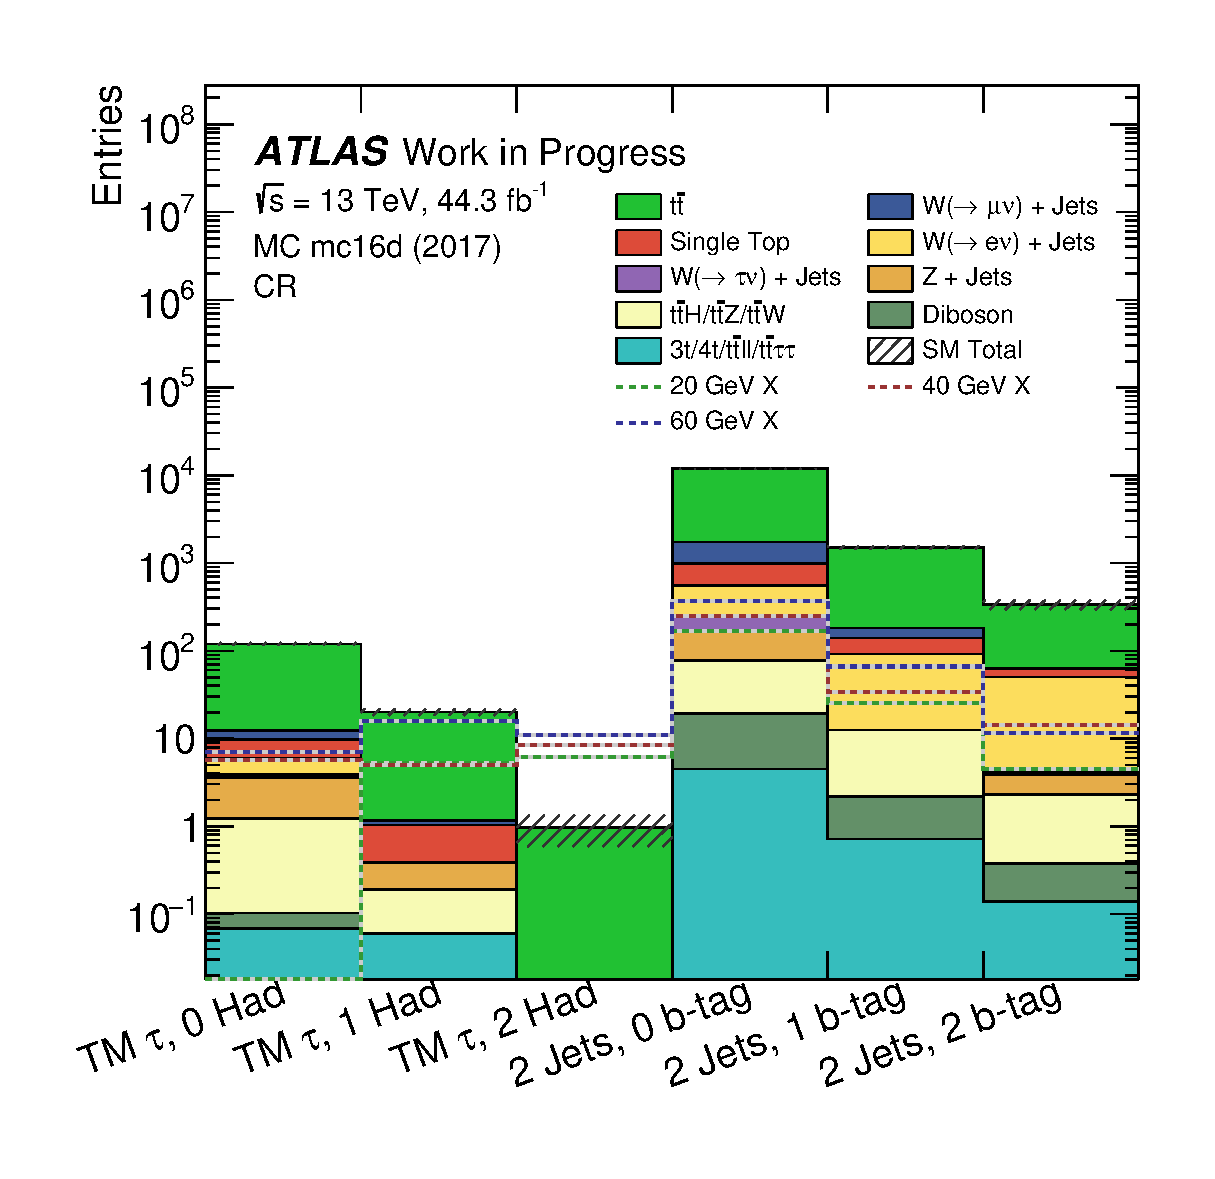
\includegraphics[width=\linewidth]{Assets/Plots/h_stack_mc16d_ditau_composition.eps}
    \caption{Composición de los objetos DiTau en la CR. Los objetos con 2 \ttaus \textit{truth} se clasifican por el número de taus en decaimiento hadrónico. Los objetos DiTau \textit{fake} originados en jets se encuentran clasificados según el número de jets identificados como b-jets (0, 1 o 2). Las muestras de señal han sido escaladas por $10^4$. Las bandas grises muestran incertezas estadísticas. El \textit{truth match} se realizó respecto al jet externo $R = 1$ del objeto DiTau.}
    \label{fig:ch5:ditau_composition}
\end{marginfigure}

\begin{table*}[t]
    \footnotesize
    \setlength{\tabcolsep}{1mm}
    \begin{tabular}{L{35mm} R{15mm}R{15mm} R{15mm}R{15mm} R{15mm}R{15mm} R{15mm}R{15mm}}
\toprule
                         & \multicolumn{2}{c}{CR}               & \multicolumn{2}{c}{CR $e$-channel}    & \multicolumn{2}{c}{CR $\mu$-channel}  & \multicolumn{2}{c}{SR}            \\
\midrule
$t\bar{t}$               & 11850.589            & ( 85.651\%)   & 4131.590          & ( 85.634\%)       & 7719.125          & ( 85.660\%)       & 583.833           & ( 77.204\%)   \\
$W(\to \mu\nu) + Jets$   & 784.409              & (  5.669\%)   & 0.000             & (  0.000\%)       & 784.409           & (  8.705\%)       & 39.071            & (  5.167\%)   \\
$Single Top$             & 498.663              & (  3.604\%)   & 173.739           & (  3.601\%)       & 324.924           & (  3.606\%)       & 26.162            & (  3.460\%)   \\
$W(\to e\nu) + Jets$     & 435.519              & (  3.148\%)   & 435.519           & (  9.027\%)       & 0.000             & (  0.000\%)       & 20.259            & (  2.679\%)   \\
$W(\to \tau\nu) + Jets$  & 87.485               & (  0.632\%)   & 22.153            & (  0.459\%)       & 65.332            & (  0.725\%)       & 3.708             & (  0.490\%)   \\
$Z(\to \mu\mu) + Jets$   & 50.881               & (  0.368\%)   & 0.010             & (  0.000\%)       & 50.871            & (  0.565\%)       & 41.298            & (  5.461\%)   \\
$t\bar{t}H$              & 26.207               & (  0.189\%)   & 9.072             & (  0.188\%)       & 17.135            & (  0.190\%)       & 2.226             & (  0.294\%)   \\
$t\bar{t}Z$              & 24.943               & (  0.180\%)   & 7.561             & (  0.157\%)       & 17.382            & (  0.193\%)       & 0.994             & (  0.131\%)   \\
$Z(\to ee) + Jets$       & 22.146               & (  0.160\%)   & 22.146            & (  0.459\%)       & 0.000             & (  0.000\%)       & 23.116            & (  3.057\%)   \\
$t\bar{t}W$              & 20.064               & (  0.145\%)   & 6.874             & (  0.142\%)       & 13.189            & (  0.146\%)       & 1.532             & (  0.203\%)   \\
$Diboson$                & 16.685               & (  0.121\%)   & 5.846             & (  0.121\%)       & 10.839            & (  0.120\%)       & 2.701             & (  0.357\%)   \\
$Z(\to \tau\tau) + Jets$ & 12.889               & (  0.093\%)   & 8.444             & (  0.175\%)       & 4.445             & (  0.049\%)       & 7.340             & (  0.971\%)   \\
$4t$                     & 1.823                & (  0.013\%)   & 0.533             & (  0.011\%)       & 1.290             & (  0.014\%)       & 0.110             & (  0.015\%)   \\
$t\bar{t}\mu\mu$         & 1.312                & (  0.009\%)   & 0.065             & (  0.001\%)       & 1.247             & (  0.014\%)       & 0.776             & (  0.103\%)   \\
$t\bar{t}\tau\tau$       & 1.312                & (  0.009\%)   & 0.394             & (  0.008\%)       & 0.918             & (  0.010\%)       & 2.594             & (  0.343\%)   \\
$t\bar{t}ee$             & 0.757                & (  0.005\%)   & 0.683             & (  0.014\%)       & 0.074             & (  0.001\%)       & 0.485             & (  0.064\%)   \\
$3t$                     & 0.256                & (  0.002\%)   & 0.079             & (  0.002\%)       & 0.177             & (  0.002\%)       & 0.019             & (  0.003\%)   \\
\textbf{Total}           & \textbf{13835.938}   &               & \textbf{4824.708} &                   & \textbf{9011.356} &                   & \textbf{756.226}  &               \\
\midrule
\SI{20}{\GeV} $X$        & 0.021                &               & 0.011             &                   & 0.010             &                   & 0.102             &               \\
\SI{40}{\GeV} $X$        & 0.032                &               & 0.016             &                   & 0.016             &                   & 0.255             &               \\
\SI{60}{\GeV} $X$        & 0.048                &               & 0.023             &                   & 0.025             &                   & 0.273             &               \\
%\midrule
%Datos                    & 12474                &               & 4210              &                   & 8264              &                   & -                 &               \\
\bottomrule
\end{tabular}

    \caption[][1em]{Composición de los fondos contaminantes y eventos de señal en la CR ($e$-channel, $\mu$-channel y canal combinado) y SR. Se utilizaron muestras MC de \texttt{mc16d}, normalizadas a la luminosidad integrada del año 2017. Trabajo en progreso.}
    \label{tbl:ch5:CR-SR_yields}
\end{table*}


\subsection{Selección de cargas en los subjets}

Como parte de la definición preliminar de la SR, se añadió un requerimiento de signos opuestos en las cargas de los subjets \textit{leading} y \textit{subleading} del objeto DiTau, asociados en los eventos de señal con el par $\tau_{\text{had}}^+\tau_{\text{had}}^-$. La adición de este corte resulta en una reducción aproximada del 50\% de los eventos de fondo en la SR (al no esperar una preferencia de signo en los eventos de fondo del SM). En la CR, por el contrario, buscamos tener el mayor número de eventos $t\bar{t}$ posibles, para aumentar el tamaño de la muestra y facilitar el análisis estadístico. Por lo tanto, es importante verificar si se puede omitir el corte sin modificar las distribuciones de las variables.

Aplicar las selecciones de signos opuestos y signos iguales de las cargas en la CR resulta en una reducción neta del número de eventos del 46.3\% y 51.7\% respectivamente, como se puede apreciar en la \cref{tbl:ch5:CR-qq_yields}. El número de eventos en las dos categorías excede la producción total en la CR. Esto es esperado, ya que la selección en el signo de las cargas reduce el número de candidatos DiTau por evento, permitiendo ahora que algunos eventos con previamente más de 1 objeto DiTau pasen el corte final $NDiTau == 1$.

\begin{table}[t]
    \footnotesize
    \setlength{\tabcolsep}{1mm}
    \begin{tabular}{L{35mm} R{15mm}R{15mm} R{15mm}R{15mm}}
\toprule
                            & \multicolumn{2}{c}{CR $q_{\text{lead}} q_{\text{sublead}} == -1$} & \multicolumn{2}{c}{CR $q_{\text{lead}} q_{\text{sublead}} == +1$} \\
\midrule
$t\bar{t}$                  & 6368.198                          & (85.678\%)                    & 5721.085                          & (85.683\%)                 \\
$W( \to \mu\nu) + Jets$     & 433.627                           & (5.834\%)                     & 364.697                           & (5.462\%)                  \\
$Single Top$                & 263.129                           & (3.540\%)                     & 244.479                           & (3.661\%)                  \\
$W( \to e\nu) + Jets$       & 253.352                           & (3.409\%)                     & 191.092                           & (2.862\%)                  \\
$W( \to \tau\nu) + Jets$    & 29.062                            & (0.391\%)                     & 58.631                            & (0.878\%)                  \\
$Z( \to \mu\mu) + Jets$     & 21.727                            & (0.292\%)                     & 30.038                            & (0.450\%)                  \\
$t\bar{t}Z$                 & 14.314                            & (0.193\%)                     & 12.394                            & (0.186\%)                  \\
$t\bar{t}H$                 & 13.860                            & (0.186\%)                     & 13.002                            & (0.195\%)                  \\
$Z( \to ee) + Jets$         & 11.487                            & (0.155\%)                     & 10.863                            & (0.163\%)                  \\
$t\bar{t}W$                 & 10.779                            & (0.145\%)                     & 9.685                             & (0.145\%)                  \\
$Diboson$                   & 8.969                             & (0.121\%)                     & 7.756                             & (0.116\%)                  \\
$Z( \to \tau\tau) + Jets$   & 2.051                             & (0.028\%)                     & 11.250                            & (0.168\%)                  \\
$4t$                        & 0.948                             & (0.013\%)                     & 0.917                             & (0.014\%)                  \\
$t\bar{t}\mu\mu$            & 0.706                             & (0.009\%)                     & 0.630                             & (0.009\%)                  \\
$t\bar{t}ee$                & 0.371                             & (0.005\%)                     & 0.375                             & (0.006\%)                  \\
$3t$                        & 0.132                             & (0.002\%)                     & 0.132                             & (0.002\%)                  \\
\textbf{Total}              & \textbf{7432.711}                 &                               & \textbf{6677.026}                 &                            \\
\bottomrule
\end{tabular}

    \caption[][1em]{Composición de los fondos contaminantes en la CR, para cargas de signos opuestos e iguales en los subjets \textit{leading} y \textit{subleading} del DiTau. Se utilizaron muestras MC de \texttt{mc16d}, normalizadas a la luminosidad integrada del año 2017. Trabajo en progreso.}
    \label{tbl:ch5:CR-qq_yields}
    \setfloatalignment{b}
\end{table}

El número total de eventos es 10.1\% más pequeño en el caso de signos iguales en los subjets, aunque no ocurre un reordenamiento significativo de los procesos de fondo. Las distribuciones cinemáticas de los objetos presentes en los eventos, exhibidas en las \cref{fig:ch5:CR-qq_distributions,fig:ch5:CR-qq_distributions_2}, también muestran un perfil similar en ambos casos. La causa de esta reducción no-uniforme en los eventos todavía no ha sido estudiada, pero podría atribuirse a una imperfecta reconstrucción de la carga de los subjets LyS del objeto DiTau.

Este primer conjunto de resultados preliminares sugiere que la adición de la selección de cargas opuestas en la CR no es necesaria. Sin embargo, estos estudios deben ser revisados una vez que se realice la re-optimización final de las definiciones de las regiones en un futuro.

\clearpage{}
\begin{figure*}[th!]
    \centering
    \setlength{\individualPlotWidth}{0.47\fulllinewidth}
    %
    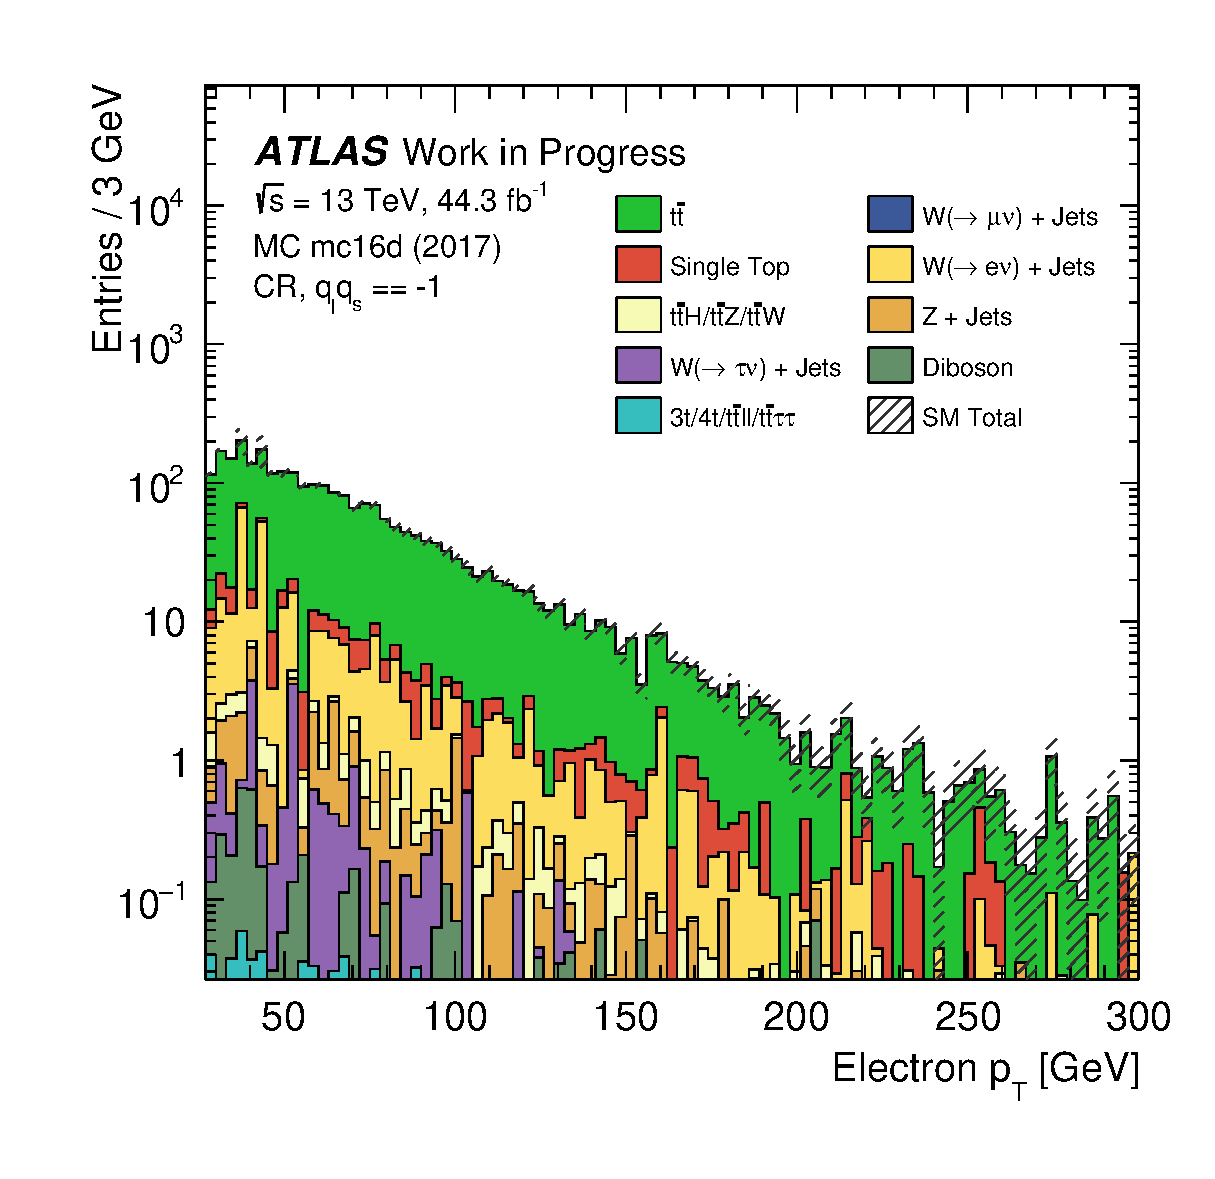
\includegraphics[width=\individualPlotWidth]{Assets/Plots/qq-sign/qq==-1/h_stack_mc16d_el_pt.eps}
    \hspace{1em}
    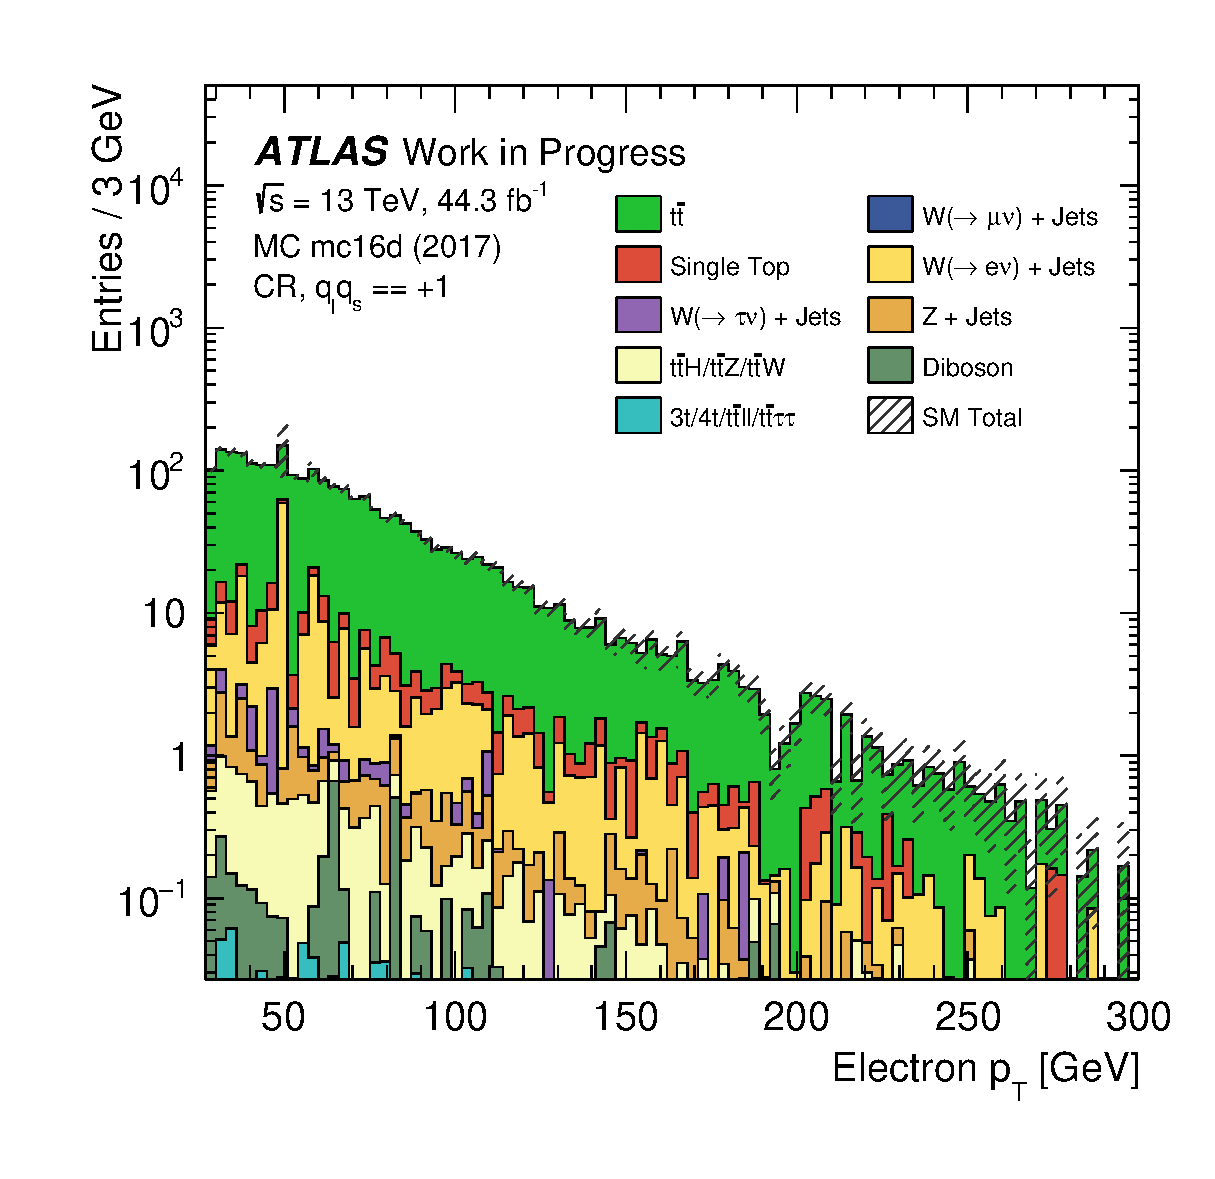
\includegraphics[width=\individualPlotWidth]{Assets/Plots/qq-sign/qq==+1/h_stack_mc16d_el_pt.eps}

    \vspace{-1.8em}
    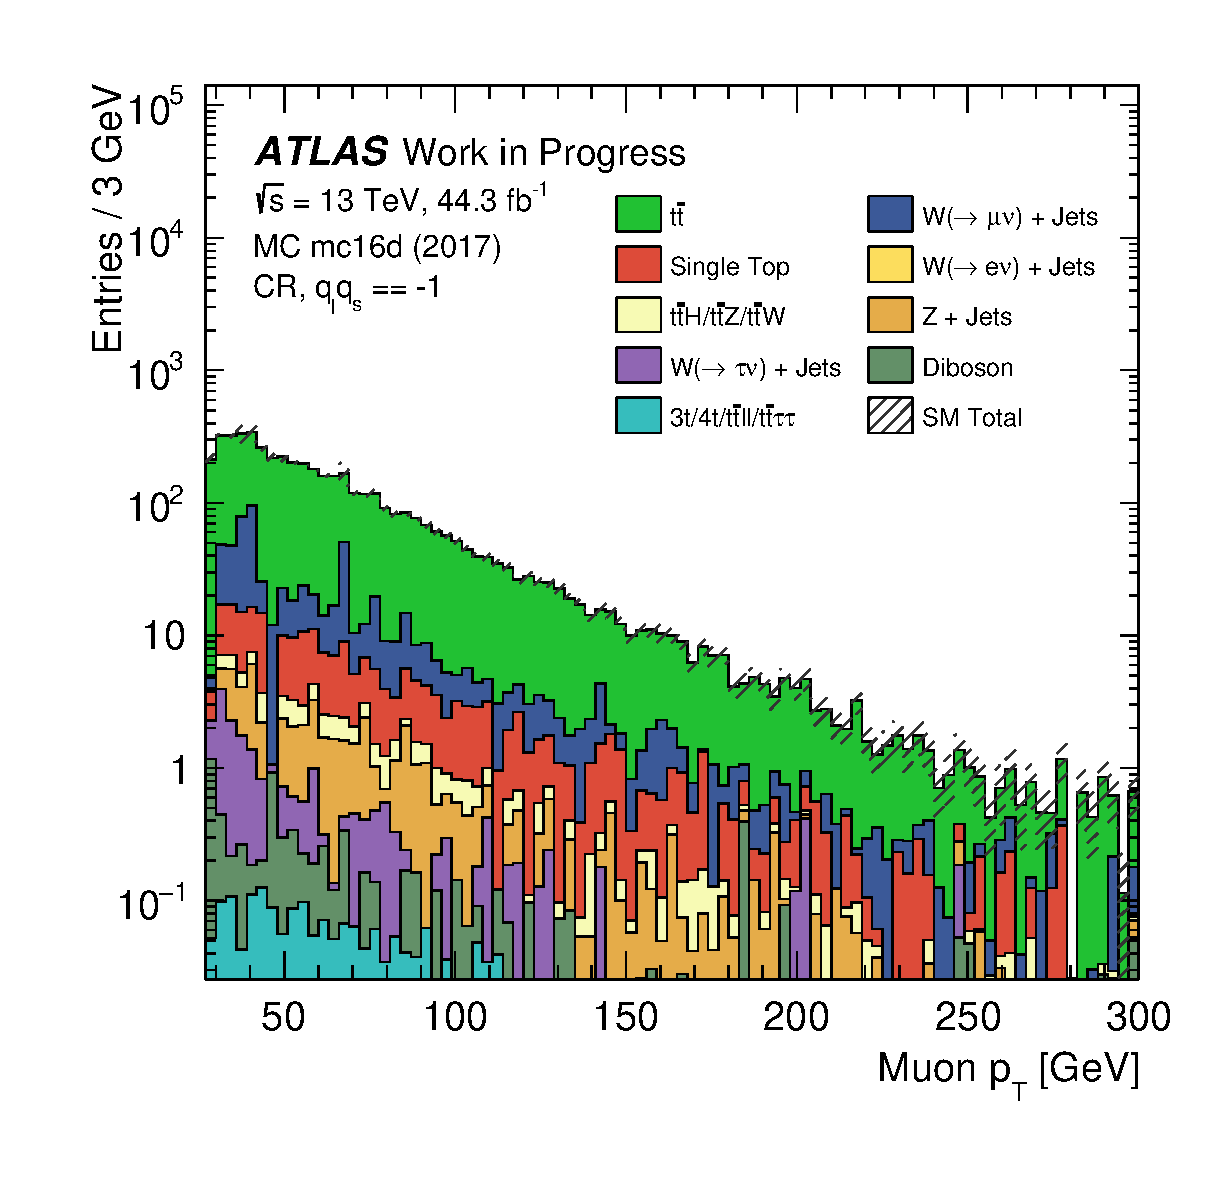
\includegraphics[width=\individualPlotWidth]{Assets/Plots/qq-sign/qq==-1/h_stack_mc16d_mu_pt.eps}
    \hspace{1em}
    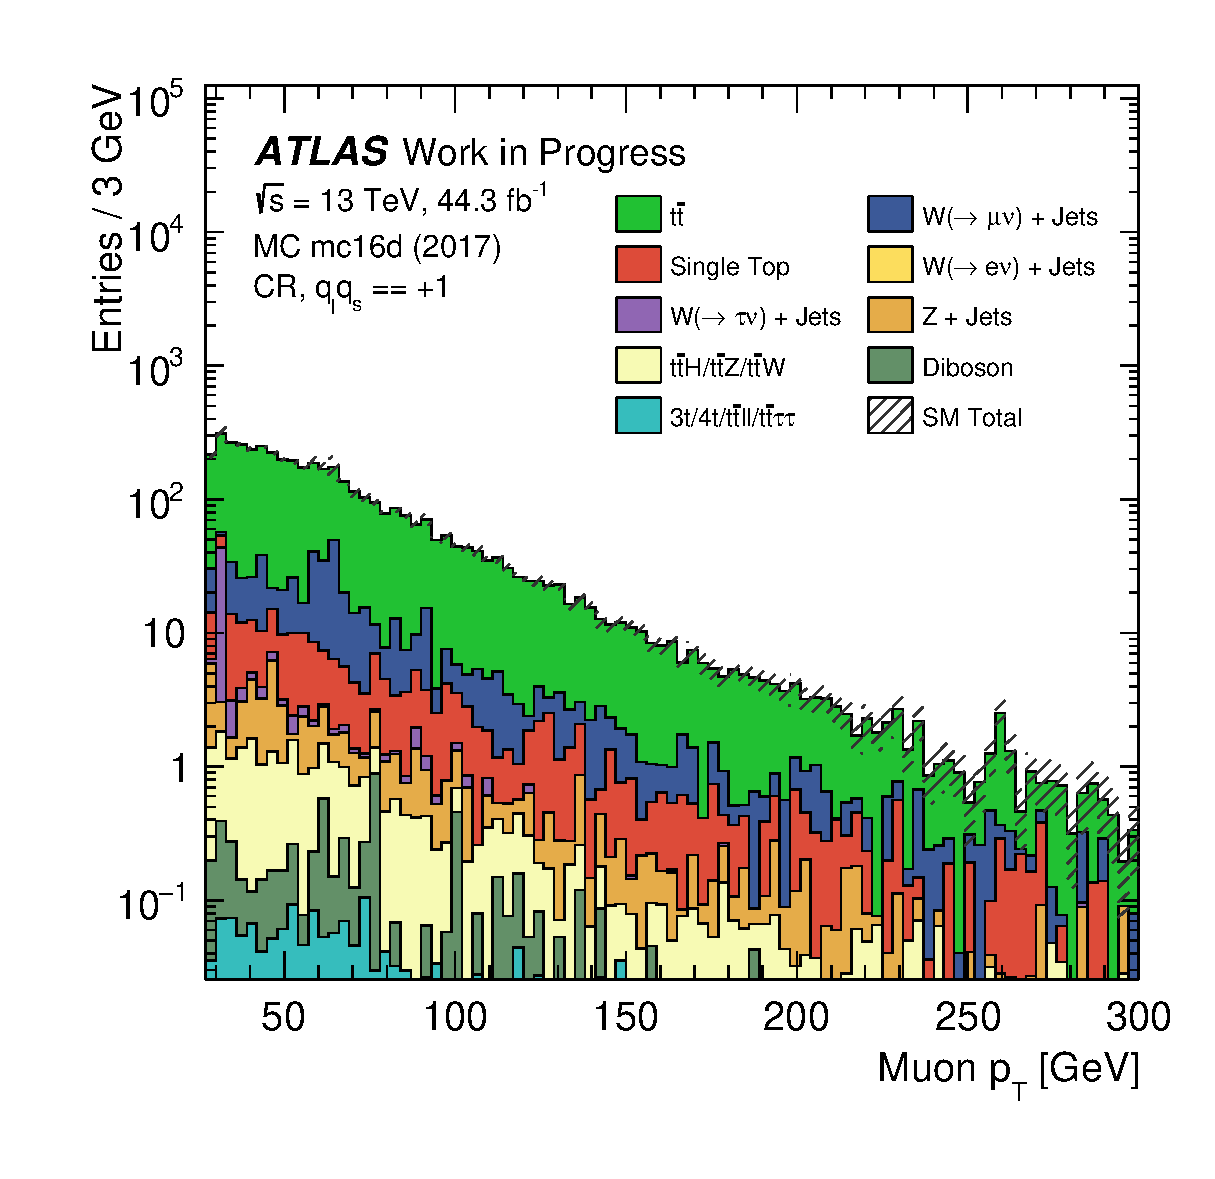
\includegraphics[width=\individualPlotWidth]{Assets/Plots/qq-sign/qq==+1/h_stack_mc16d_mu_pt.eps}

    \vspace{-1.8em}
    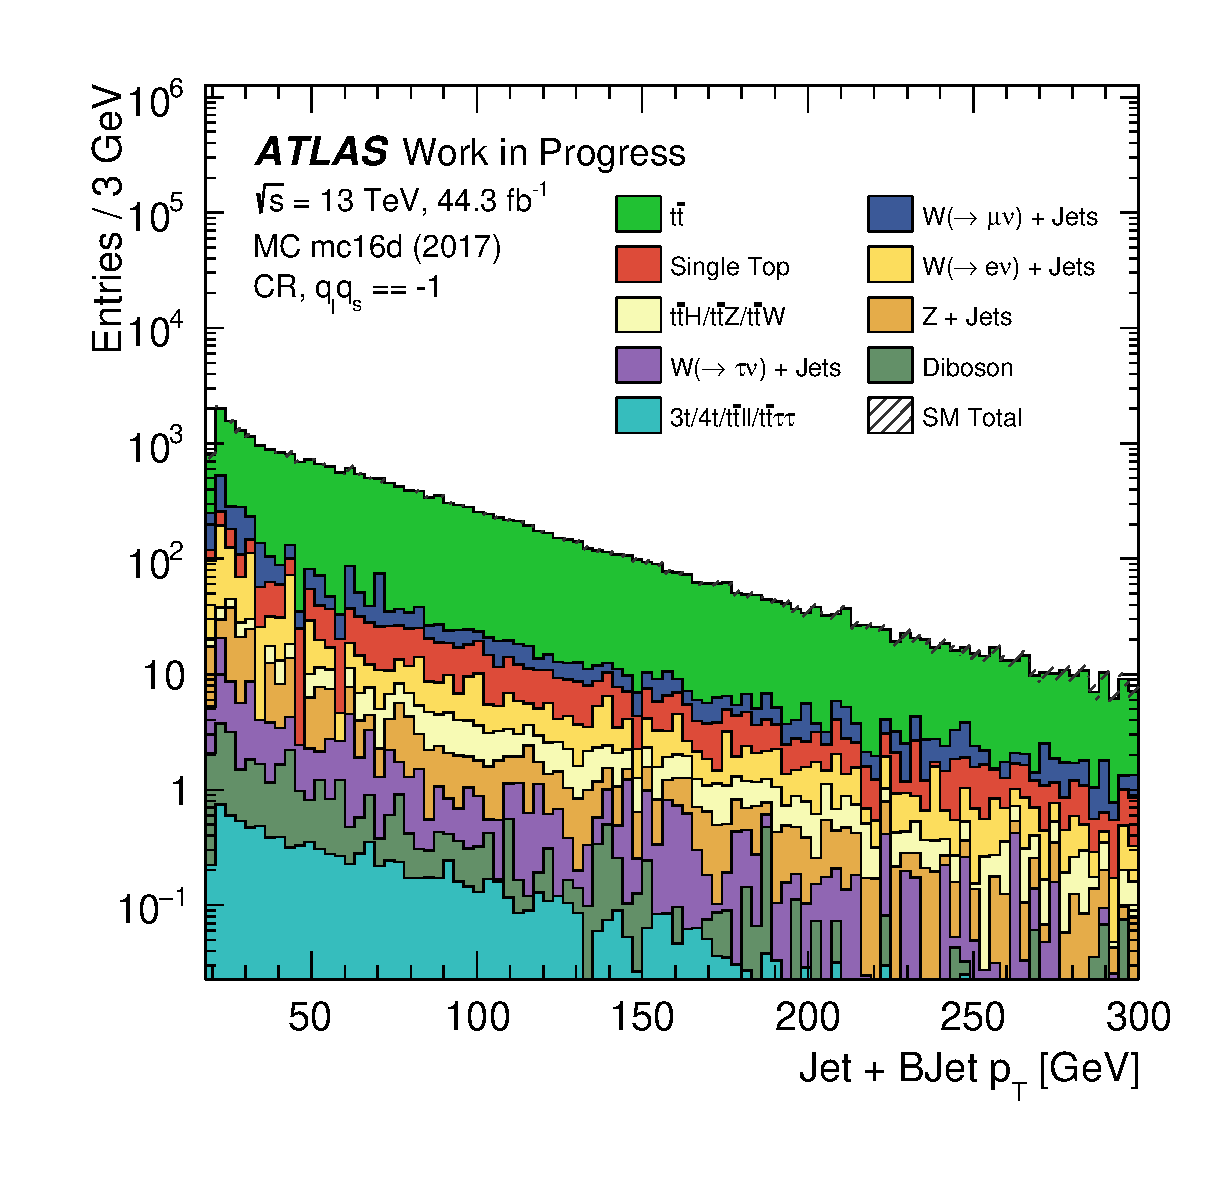
\includegraphics[width=\individualPlotWidth]{Assets/Plots/qq-sign/qq==-1/h_stack_mc16d_jet_tot_pt.eps}
    \hspace{1em}
    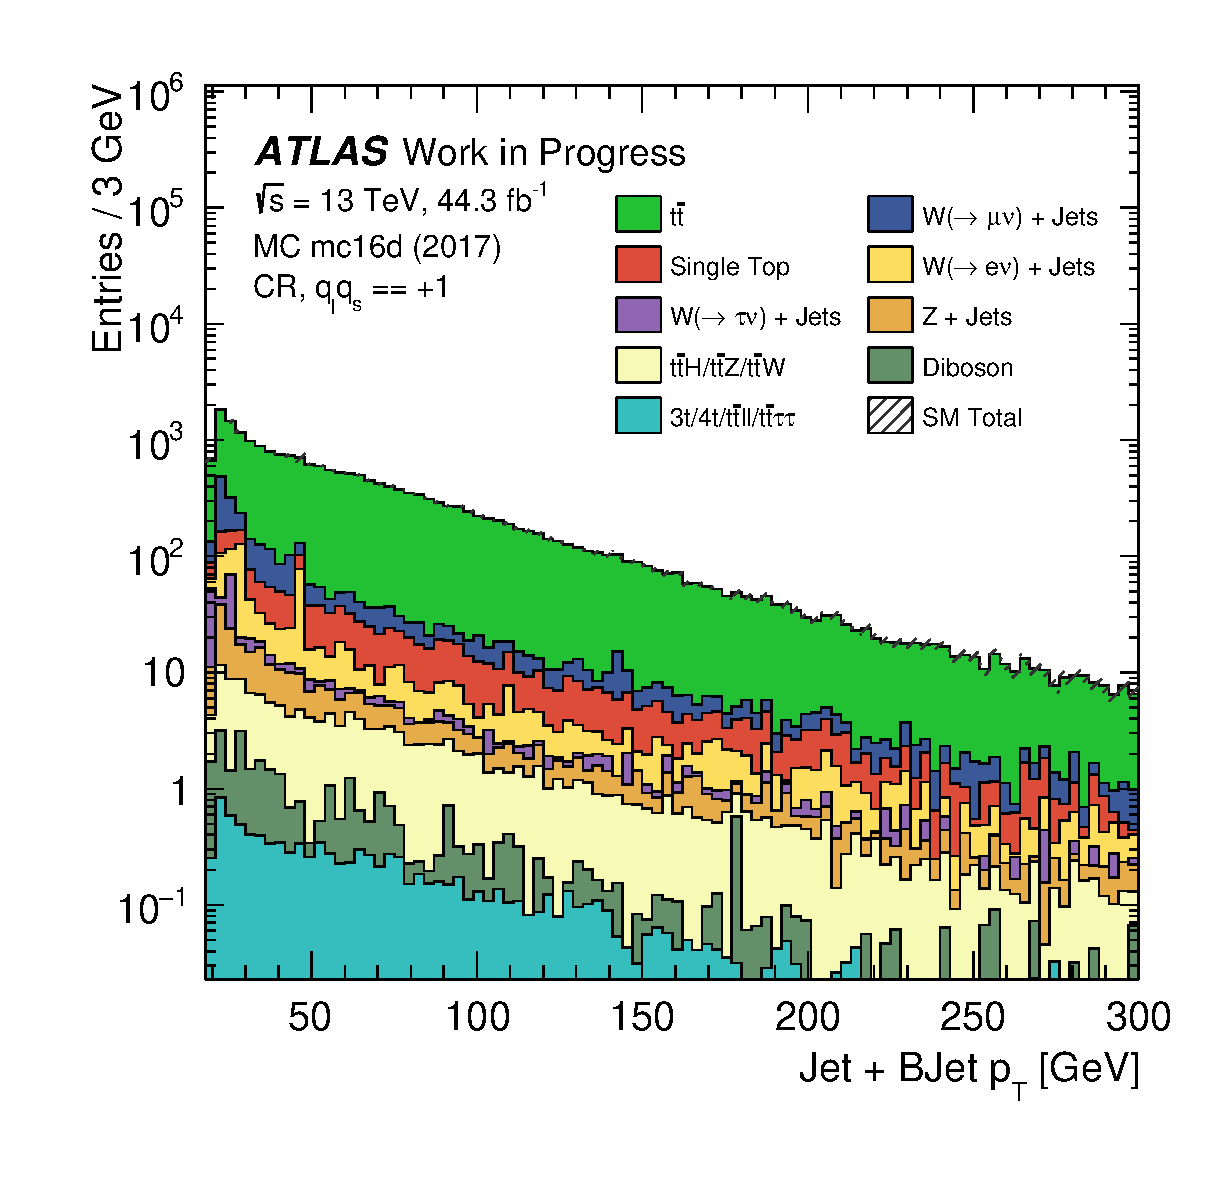
\includegraphics[width=\individualPlotWidth]{Assets/Plots/qq-sign/qq==+1/h_stack_mc16d_jet_tot_pt.eps}

    \vspace{-1em}
    \fullwidthCaption{Distribuciones cinemáticas de $p_T$ de los leptones y (b)jets en la CR, para cargas de signos opuestos (izquierda) e iguales (derecha) en los subjets \textit{leading} y \textit{subleading} del DiTau. El último bin incluye \textit{overflows}.}
    \label{fig:ch5:CR-qq_distributions}
\end{figure*}

\let\oldthefigure\thefigure
%\renewcommand{\thefigure}{\oldthefigure \ (Cont.)}
\begin{figure*}[th!]
    \centering
    \setlength{\individualPlotWidth}{0.47\fulllinewidth}
    %
    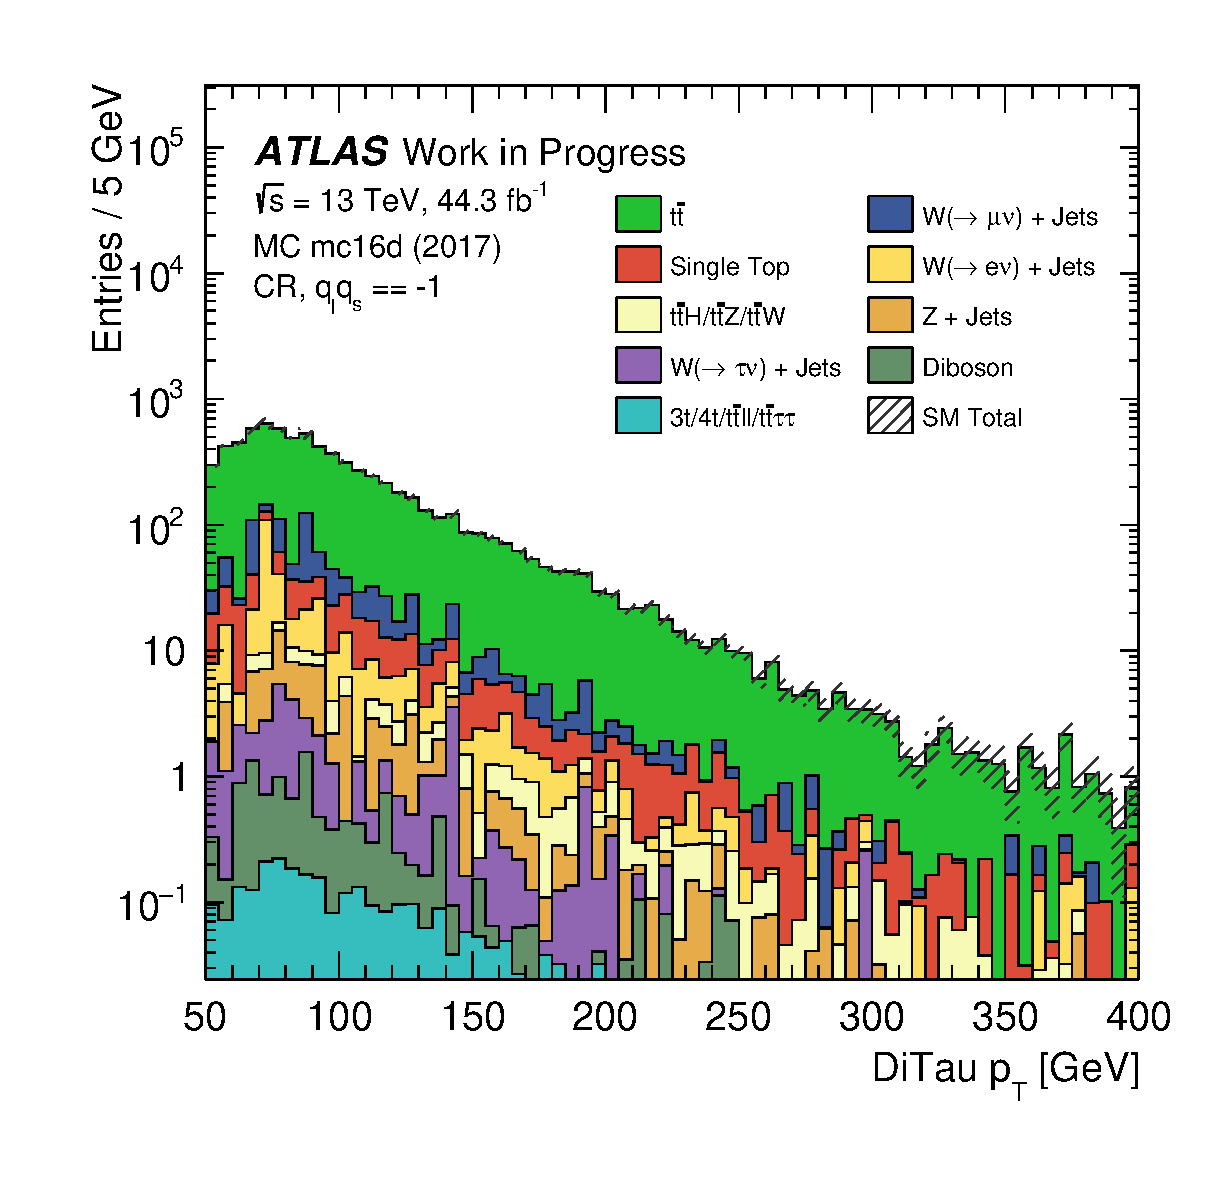
\includegraphics[width=\individualPlotWidth]{Assets/Plots/qq-sign/qq==-1/h_stack_mc16d_ditau_pt.eps}
    \hspace{1em}
    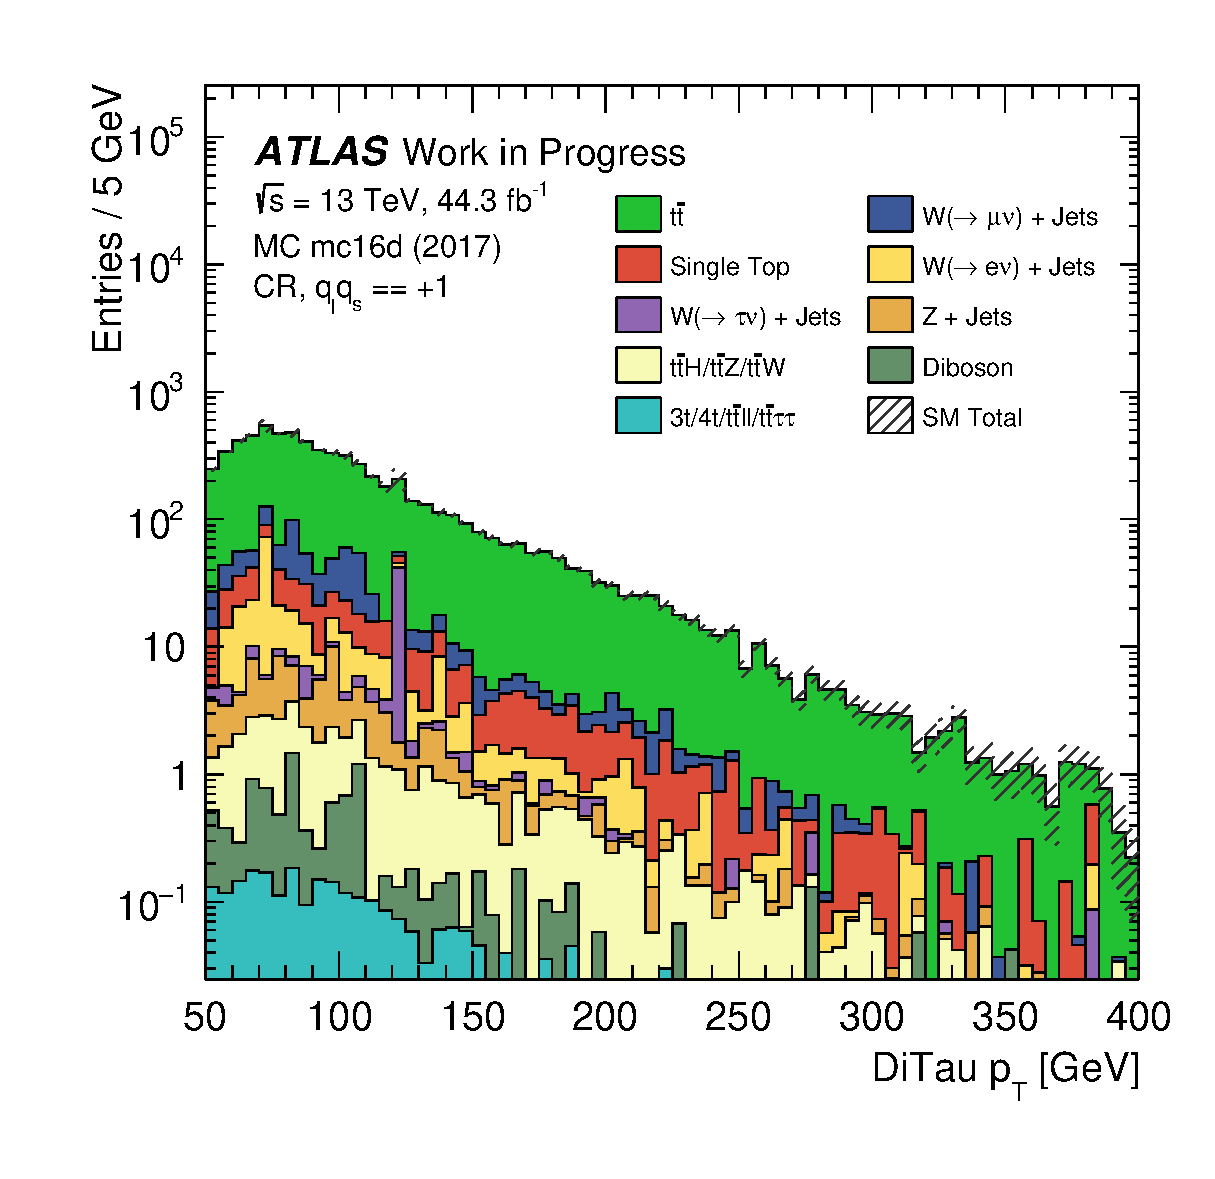
\includegraphics[width=\individualPlotWidth]{Assets/Plots/qq-sign/qq==+1/h_stack_mc16d_ditau_pt.eps}

    \caption{Distribuciones cinemáticas de $p_T$ de los DiTaus en la CR, para cargas de signos opuestos (izquierda) e iguales (derecha) en los subjets \textit{leading} y \textit{subleading} del DiTau. El último bin incluye \textit{overflows}.}
    \label{fig:ch5:CR-qq_distributions_2}
    %\ContinuedFloat
\end{figure*}
%\renewcommand{\thefigure}{\oldthefigure}





\noFBSection[Comparación con los datos experimentales y estimación de \texorpdfstring{$\mu_{t\overline{t}}$}{mu\_ttbar}]{Comparación con los datos experimentales y estimación de \texorpdfstring{$\mu_{t\bar{t}}$}{mu\_ttbar}}

La \cref{fig:ch5:h_results} muestra las distribuciones de $p_T$ de eventos de datos y simulaciones de los fondos del SM para los objetos DiTau y leptones en la CR. Al considerarse solo eventos con un único leptón, las variables $p_T^{e}$ y $p_T^{\mu}$ contienen solo eventos en el \textit{$e$-channel} y \textit{$\mu$-channel} respectivamente. 

En todas las variables y canales se observa un menor número de eventos en los datos, evidenciando la necesidad de una corrección a la predicción de los modelos en las simulaciones. Las figuras exhiben una buena concordancia entre la forma de la distribución de los datos y los perfiles simulados en los procesos del SM, permaneciendo la diferencia aproximadamente constante en todo el rango de las variables. En consecuencia, se procederá a obtener una corrección global en todo el rango de las variables en cuestión.

\begin{figure*}[t]
    \vspace{-1.4em}
    \centering
    \setlength{\individualPlotWidth}{0.434\fulllinewidth}
    %
    \begin{minipage}{0.91\fulllinewidth}
        \raggedright
        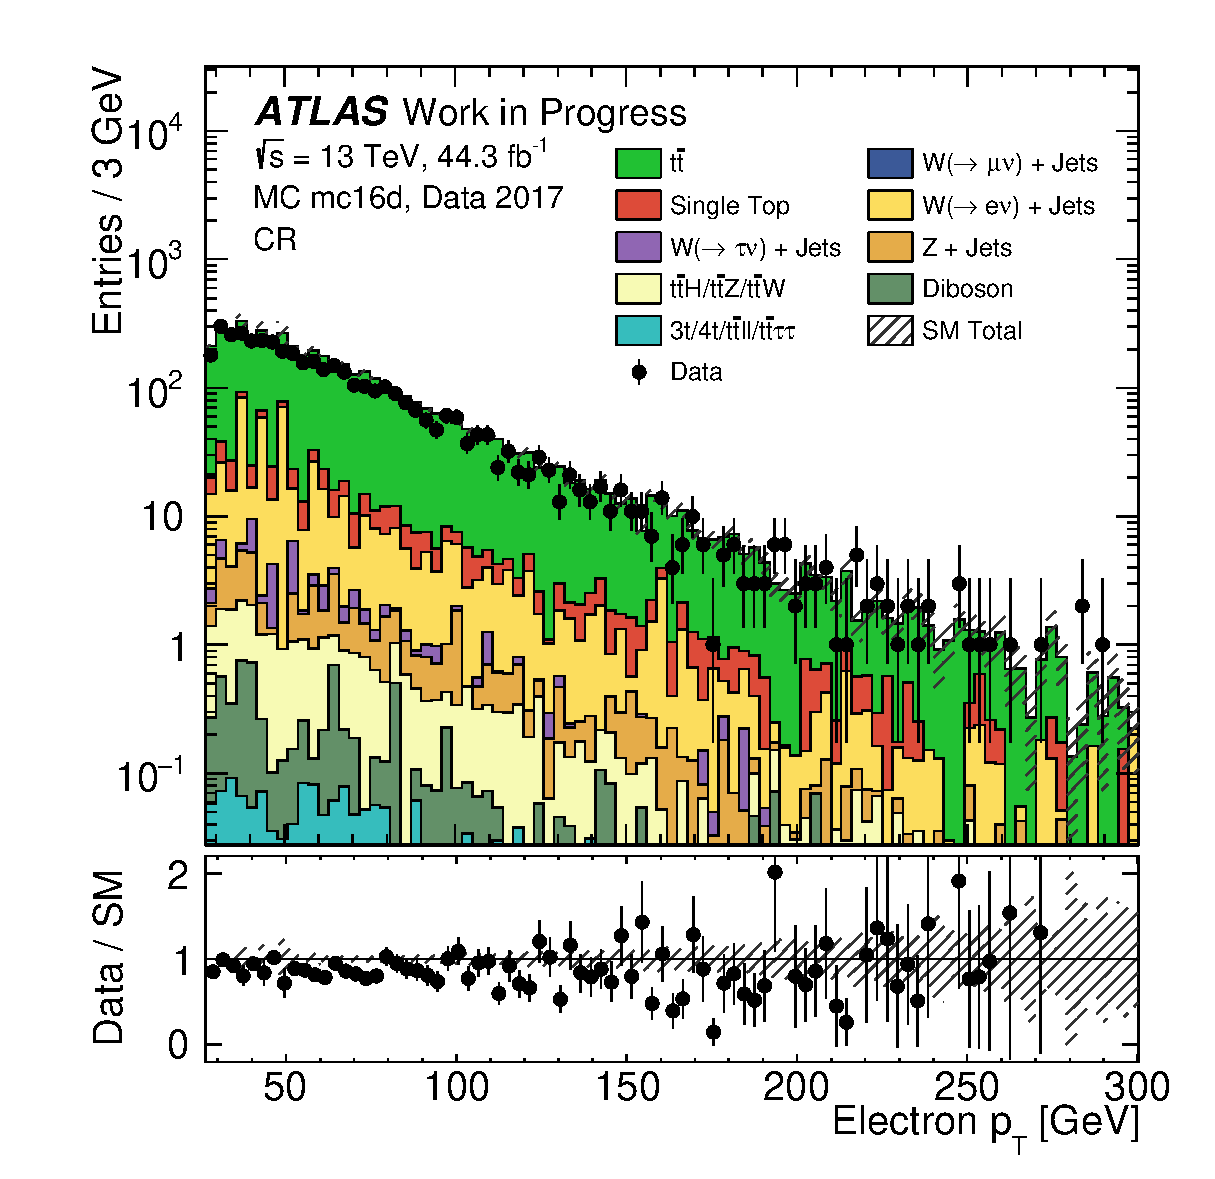
\includegraphics[width=\individualPlotWidth]{Assets/Plots/withData/h_stack_mc16d_data17_el_pt.eps}
        \hspace{1em}
        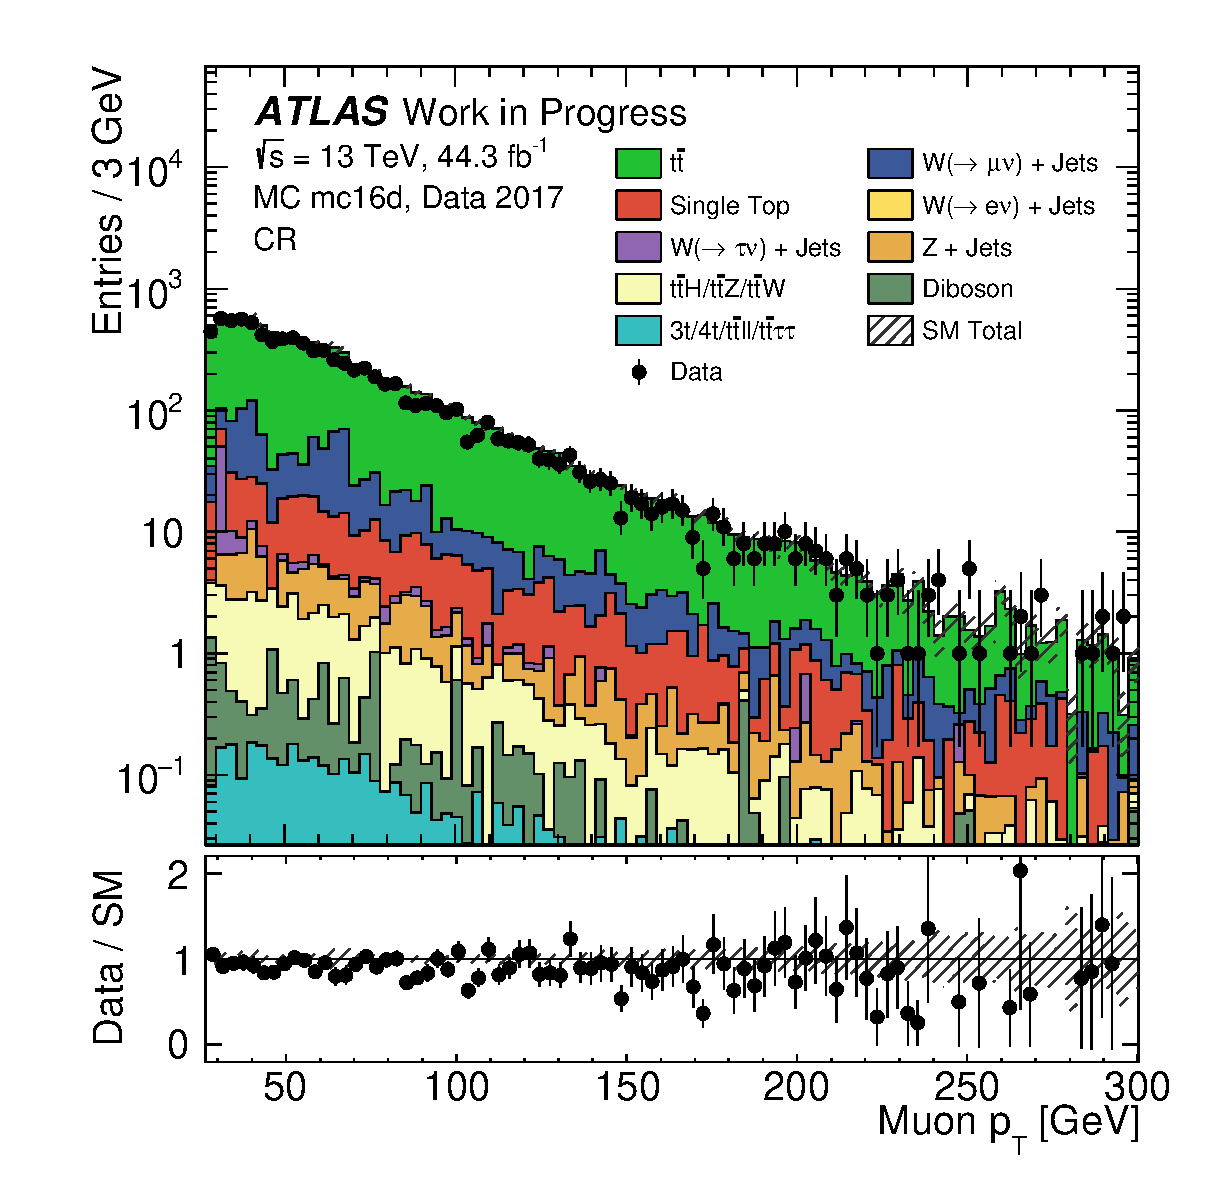
\includegraphics[width=\individualPlotWidth]{Assets/Plots/withData/h_stack_mc16d_data17_mu_pt.eps}

        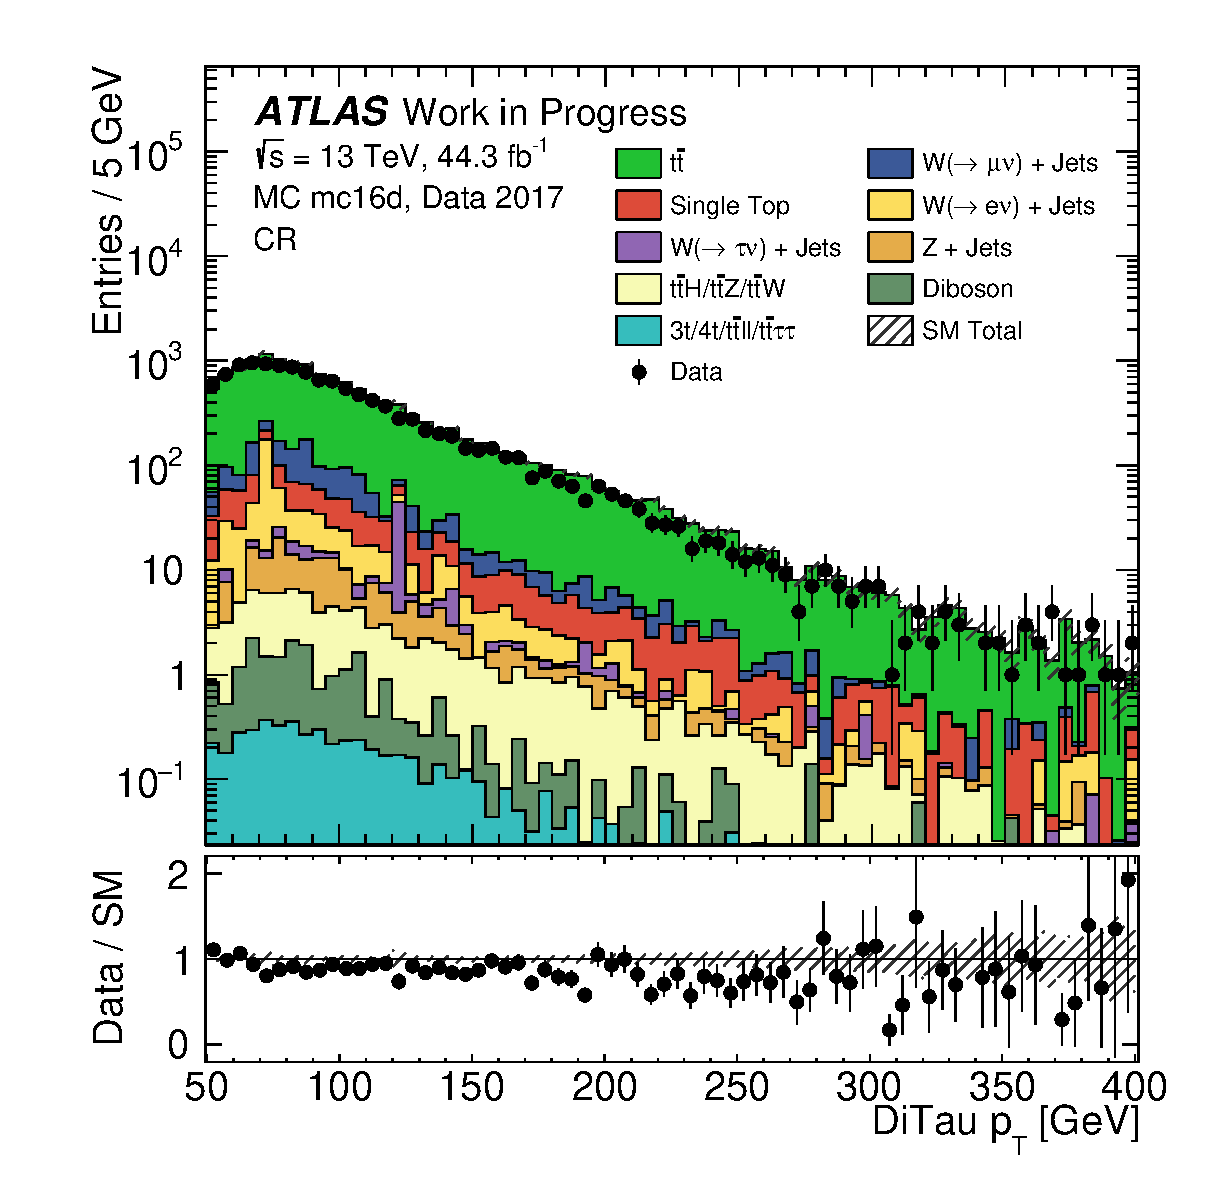
\includegraphics[width=\individualPlotWidth]{Assets/Plots/withData/h_stack_mc16d_data17_ditau_pt.eps}
    \end{minipage}

    \caption[][-8em]{Distribuciones cinemáticas de $p_T$ de los leptones y DiTaus en la CR. Las gráficas $p_T^e$ y $p_T^\mu$ corresponden al $e$-channel y $\mu$-channel respectivamente. Las bandas grises en el panel superior e inferior muestran incertezas estadísticas en las simulaciones MC. El último bin incluye \textit{overflows}.}
    \label{fig:ch5:h_results}
\end{figure*}

La determinación final de los factores de transferencia en un análisis es realizada mediante un ajuste multivariable simultáneo en todas las regiones de control, validación y señal. Sin embargo, podemos hacer un cálculo estimativo que nos permite obtener un valor preliminar de $\mu_{t\bar{t}}$ como
\[ \mu_{t\bar{t}} = \frac{N(\text{Datos}) - N(\text{MC} \neq t\bar{t})}{N(\text{MC} = t\bar{t})}, \]
donde $N(\text{Datos})$ es el número de eventos en los datos en la CR, $N(\text{MC} = t\bar{t})$ es el número de eventos MC contribuidos por el fondo $t\bar{t}$ en la CR y $N(\text{MC} \neq t\bar{t})$ es el número total de eventos MC de fondo no producidos por $t\bar{t}$ en la CR (\cref{tbl:ch5:ttbar_mu}). El canal combinado, incluyendo todos los eventos seleccionados en la CR, posee un valor preliminar del factor de transferencia de $\mu_{t\bar{t}}^{\text{Combined}} = 0.885(13)$. El canal muónico alcanza un mejor acuerdo entre las simulaciones del SM y los datos, donde $\mu_{t\bar{t}}^{\mu-\text{channel}} = 0.903(16)$, comparado con $\mu_{t\bar{t}}^{e-\text{channel}} = 0.851(22)$ en el canal electrónico.

La discrepancia entre los canales leptónicos no ha sido todavía estudiada en profundidad, aunque la principal hipótesis la atribuye a diferencias en la eficiencia de los triggers electrónicos y muónicos utilizados en el análisis. Si bien no se han considerado incertezas sistemáticas en las simulaciones de MC, esta diferencia significativa, excediendo la incerteza estadística, sugiere un tratamiento por separado del $e$-channel y el $\mu$-channel en la búsqueda. Si se opta por la estrategia inicial de un único canal, la diferencia sería incorporada como una incerteza sistemática adicional al análisis.

La \cref{fig:ch5:h_corrected} contiene las distribuciones cinemáticas de los leptones, DiTaus y $E_T^{\text{miss}}$, corregidas en cada canal. Nuevamente, no se observan diferencias significativas en los perfiles de las distribuciones entre datos y eventos simulados. Es importante recordar que las estimaciones aquí presentadas no incluyen las contribuciones del peso de los objetos DiTau, definido en la \cref{sec:ch4:processing}. Por lo tanto, se podría potencialmente alcanzar un mejor acuerdo entre los datos y las simulaciones, resultando en factores de transferencia más próximos a la unidad.

\begin{table}[bh!]
    \centering
    \small
    \begin{tabular}{lcccc}
\toprule
                  & $N(\text{MC Total})$ & $N(\text{MC} \ t\bar{t})$ & $N(\text{Datos})$ & $\mu_{t\bar{t}}$ preliminar   \\
\midrule
Canal combinado   & 13836                & 11851                     & 12474             & $0.885 \pm 0.013$             \\
Canal electrónico & 4825                 & 4132                      & 4210              & $0.851 \pm 0.022$             \\
Canal muónico     & 9011                 & 7719                      & 8264              & $0.903 \pm 0.016$             \\
\bottomrule
\end{tabular}
    \caption[][-2em]{Estimación preliminar de los factores de transferencia $\mu_{t\bar{t}}$ para la CR del fondo $t\bar{t}$ en el canal electrónico (solo eventos con trigger en un electrón), el canal muónico (solo eventos con trigger en un muón) y el canal combinado (eventos con trigger en un electrón o un muón). Trabajo en progreso.}
    \label{tbl:ch5:ttbar_mu}
\end{table}

\clearpage{}
\begin{figure*}[th!]
    \centering
    \setlength{\individualPlotWidth}{0.434\fulllinewidth}
    %
    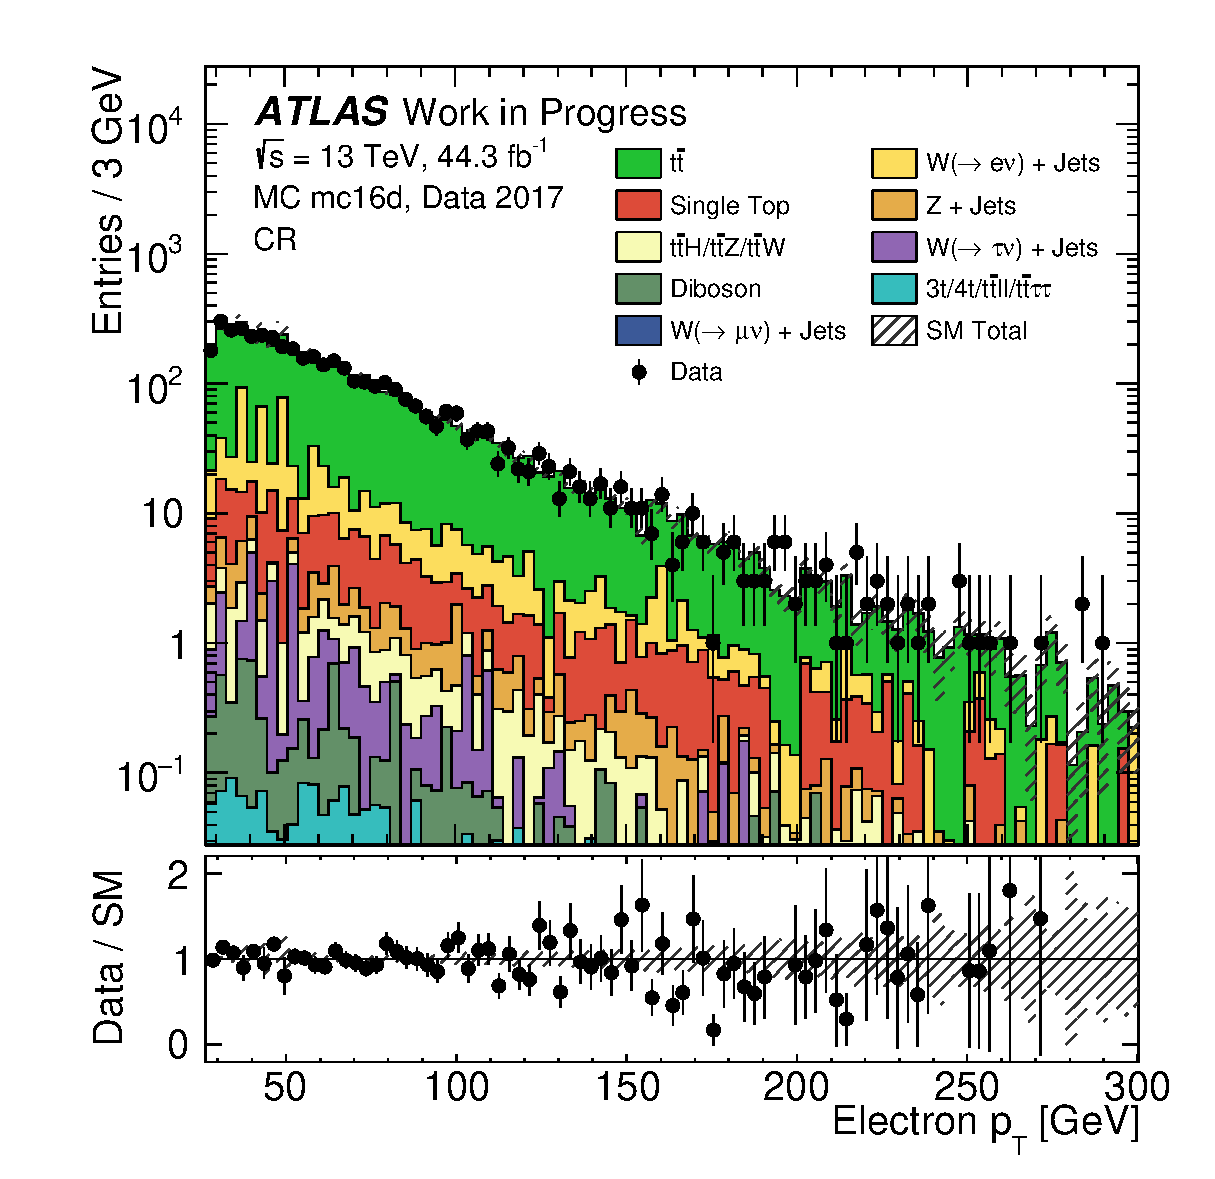
\includegraphics[width=\individualPlotWidth]{Assets/Plots/withTF/e-channel/h_stack_mc16d_data17_el_pt.eps}
    \hspace{1em}
    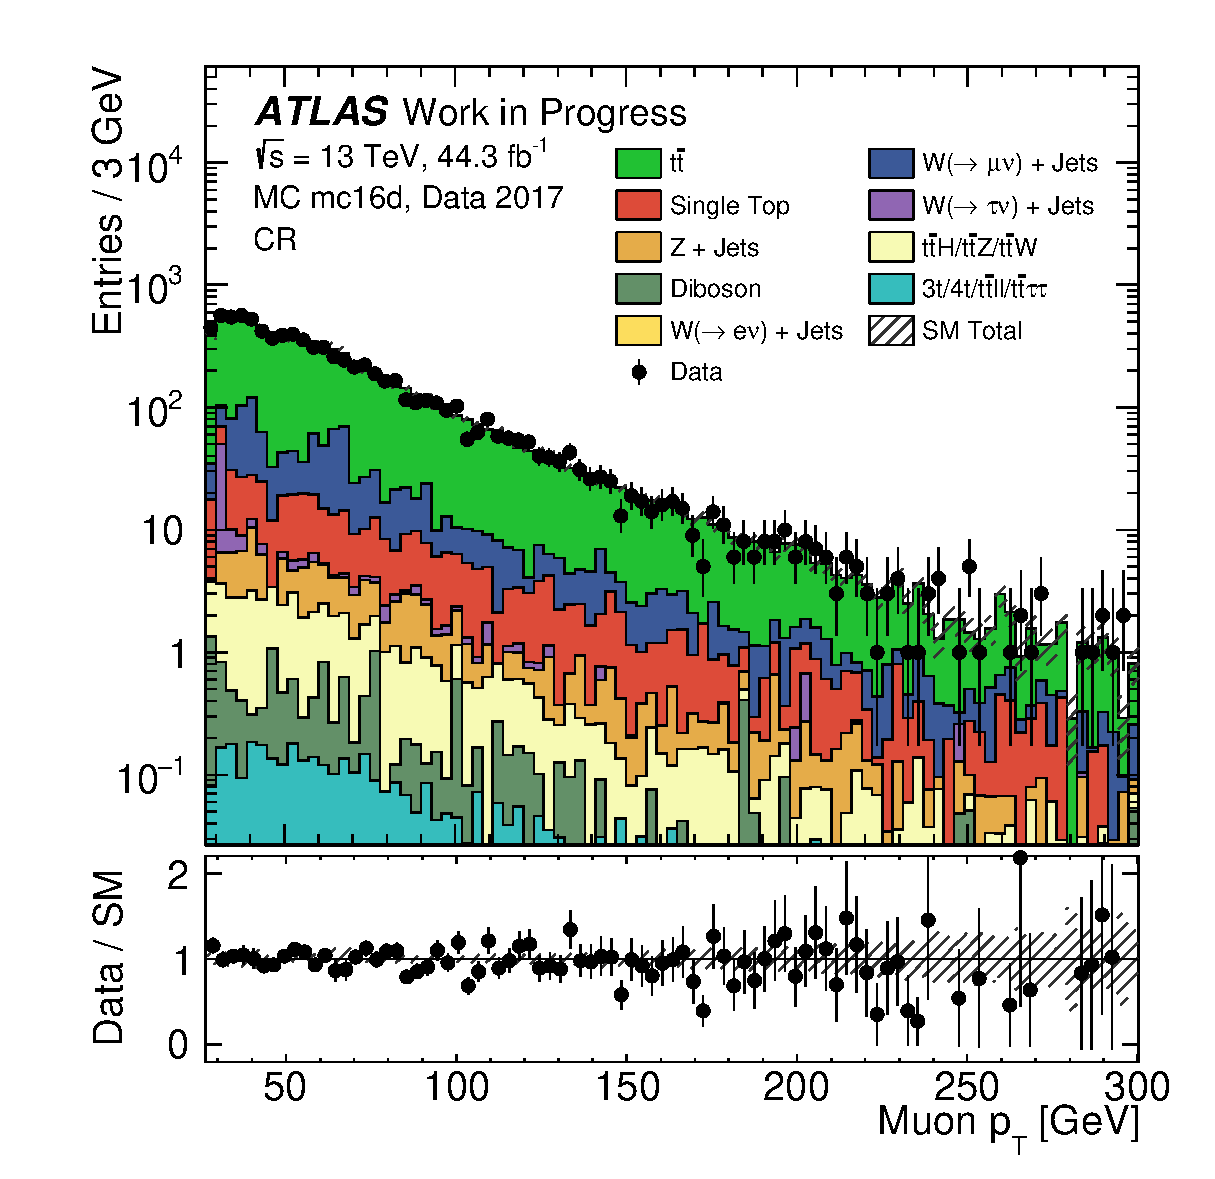
\includegraphics[width=\individualPlotWidth]{Assets/Plots/withTF/mu-channel/h_stack_mc16d_data17_mu_pt.eps}
    
    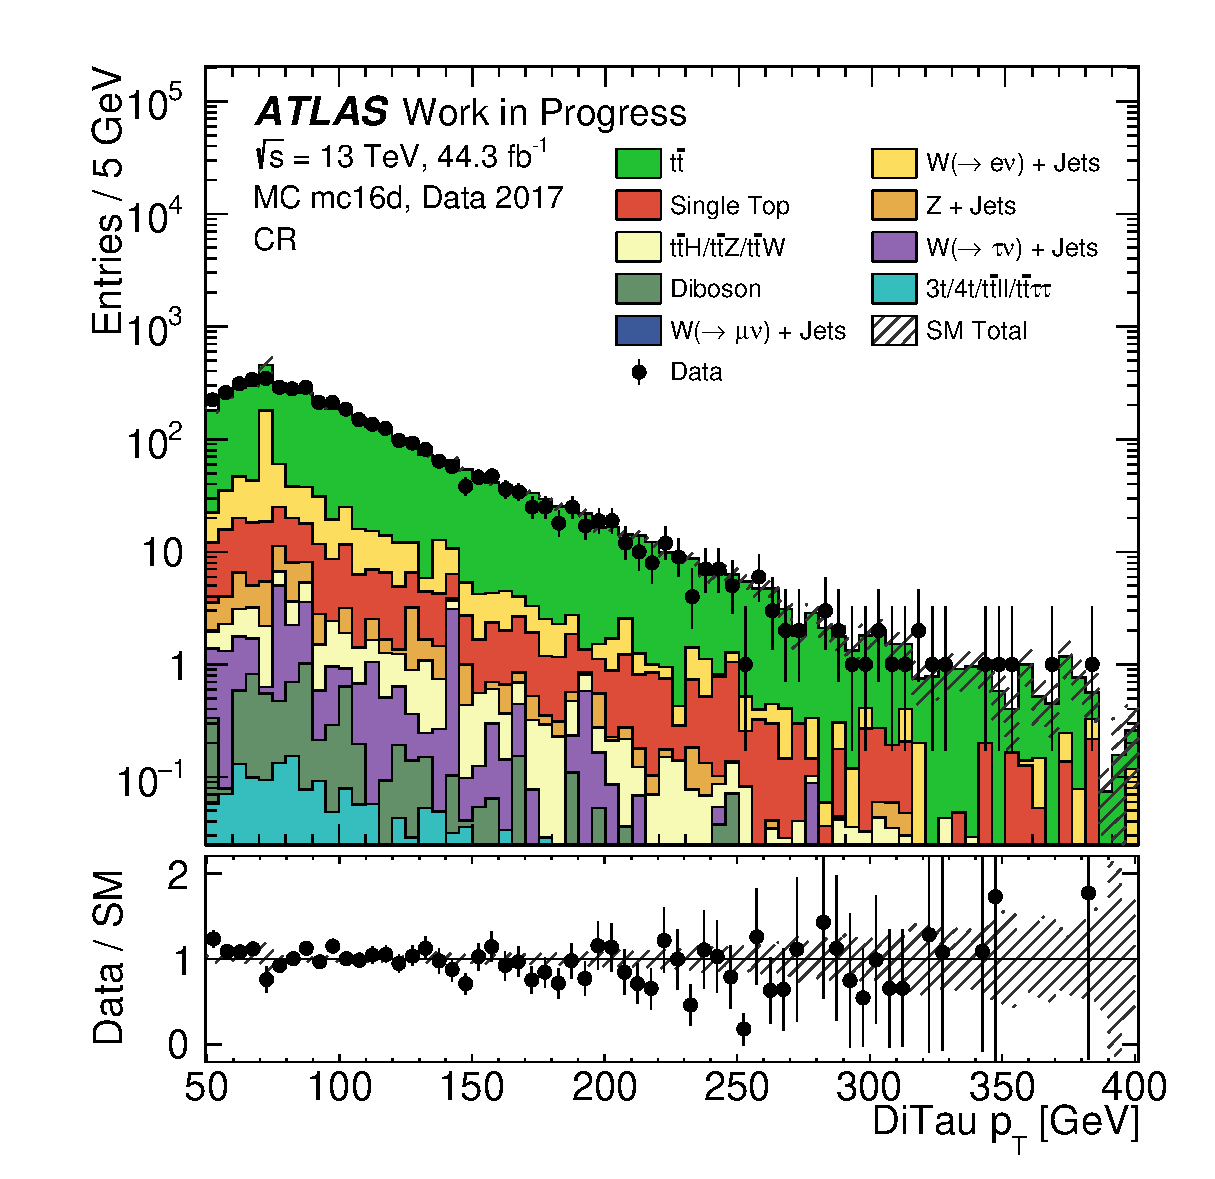
\includegraphics[width=\individualPlotWidth]{Assets/Plots/withTF/e-channel/h_stack_mc16d_data17_ditau_pt.eps}
    \hspace{1em}
    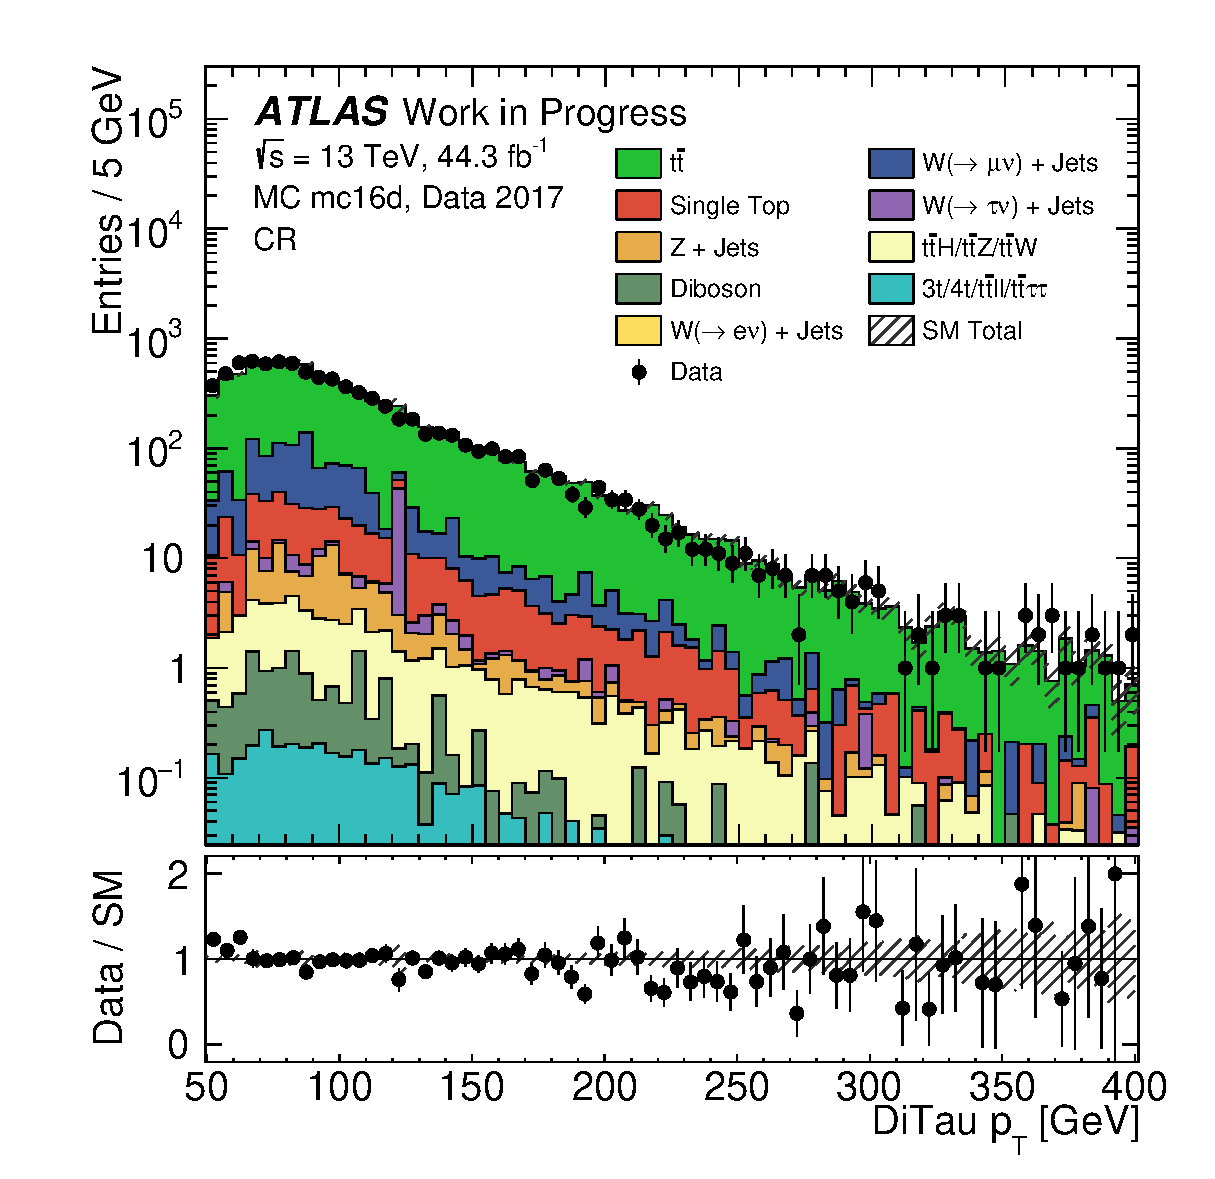
\includegraphics[width=\individualPlotWidth]{Assets/Plots/withTF/mu-channel/h_stack_mc16d_data17_ditau_pt.eps}

    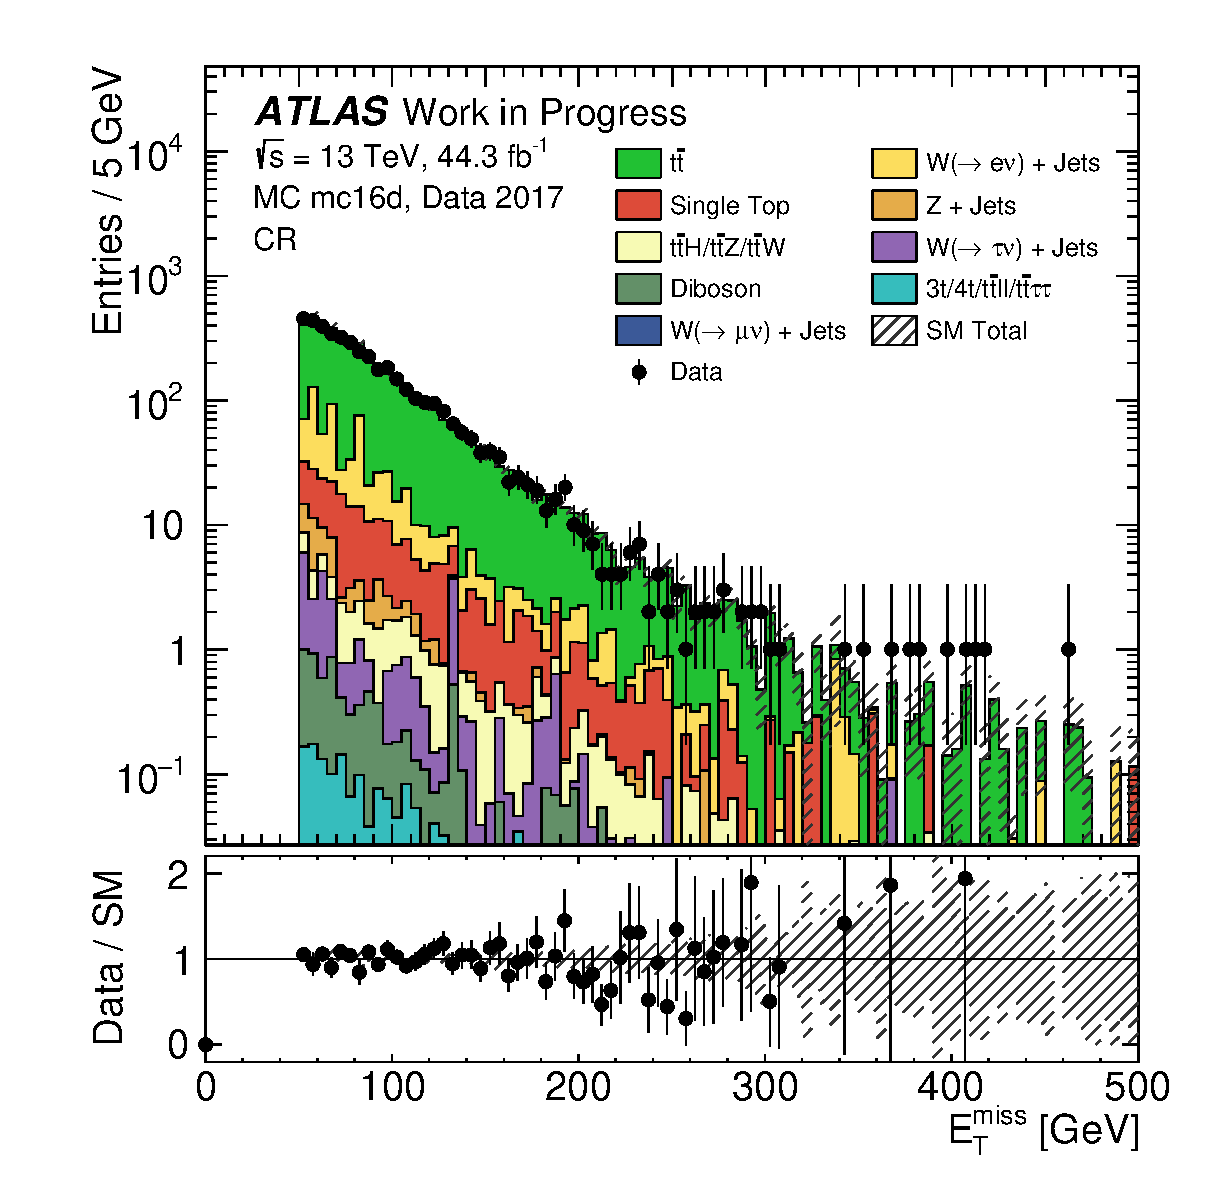
\includegraphics[width=\individualPlotWidth]{Assets/Plots/withTF/e-channel/h_stack_mc16d_data17_met_et.eps}
    \hspace{1em}
    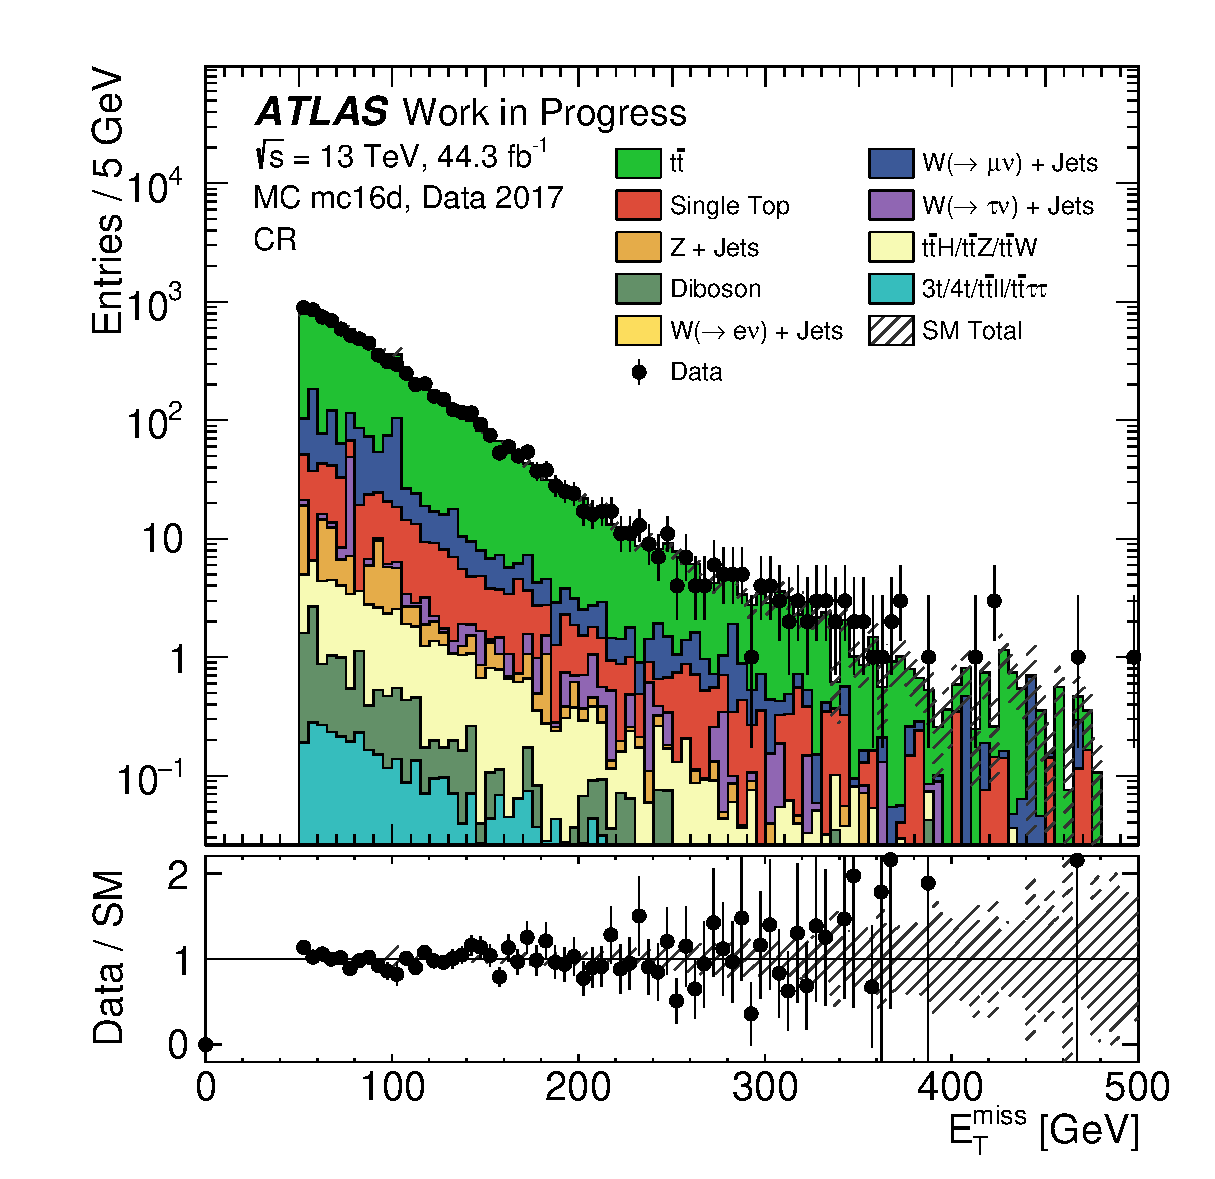
\includegraphics[width=\individualPlotWidth]{Assets/Plots/withTF/mu-channel/h_stack_mc16d_data17_met_et.eps}

    \fullwidthCaption{Distribuciones cinemáticas de $p_T$ de los leptones, DiTau y $E_T^{\text{miss}}$ del canal electónico (izquierda) y el canal muónico (derecha), corregidas con los factores de normalización $\mu_{t\bar{t}}^{e/\mu-\text{channel}}$. Las bandas grises en el panel superior e inferior muestran incertezas estadísticas en las simulaciones MC. El último bin incluye \textit{overflows}.}
    \label{fig:ch5:h_corrected}
\end{figure*}

\cleardoublepage{}